\documentclass[fleqn,10pt]{wlscirep}
\usepackage{graphicx}
\usepackage{pdfpages}
\usepackage{longtable}
\usepackage{listings}
\usepackage{multicol}
\usepackage{caption}
\usepackage{subcaption}
\usepackage{breakcites}
\usepackage{indentfirst}
\usepackage[hyphens]{url}
\lstset{
basicstyle=\small\ttfamily,
columns=flexible,
breaklines=true
}
\newcommand{\beginsupplement}{%
    \setcounter{table}{0}
    \renewcommand{\thetable}{S\arabic{table}}%
    \setcounter{figure}{0}
    \renewcommand{\thefigure}{S\arabic{figure}}%
   }

\title{Comparative Annotation Toolkit (CAT) - simultaneous clade and personal genome annotation}

\author[1]{Ian T. Fiddes}
\author[1,*]{Joel Armstrong}
\author[1,*]{Mark Diekhans}
\author[2,*]{Stefanie Nachtweide}
\author[3]{Zev N. Kronenberg}
\author[3,5]{Jason G. Underwood}
\author[3,4]{David Gordon}
\author[1]{Dent Earl}
\author[6]{Thomas Keane}
\author[3,4]{Evan E. Eichler}
\author[1]{David Haussler}
\author[2]{Mario Stanke}
\author[1,+]{Benedict Paten}
\affil[1]{Genomics Institute, University of California Santa Cruz and Howard Hughes Medical Institute, Santa Cruz, CA 95064, USA}
\affil[2]{Institute of Mathematics and Computer Science, University of Greifswald, Domstraße 11, Germany}
\affil[3]{Department of Genome Sciences, University of Washington School of Medicine, Seattle, WA 98195, USA}
\affil[4]{Howard Hughes Medical Institute, University of Washington, Seattle, WA 98195, USA}
\affil[5]{Pacific Biosciences of California, Inc., Menlo Park, CA 94025, USA}
\affil[6]{European Bioinformatics Institute, Wellcome Genome Campus, Hinxton CB10 1SD, UK}

\affil[+]{Corresponding author. Email: bpaten@ucsc.edu}

\affil[*]{These authors contributed equally to this work}

\keywords{Comparative Annotation, Whole-Genome Alignment, Genome Annotation, Comparative Genomics}

\begin{abstract}
The recent introductions of low-cost, long-read, and read-cloud sequencing technologies coupled with intense efforts to develop efficient algorithms have made affordable, high-quality \textit{de novo} sequence assembly a realistic proposition. The result is an explosion of new, ultra-contiguous genome assemblies. To compare these genomes we need robust methods for genome annotation. We describe the fully open source Comparative Annotation Toolkit (CAT), which provides a flexible way to simultaneously annotate entire clades and identify orthology relationships. We show that CAT can be used to improve annotations on the rat genome, annotate the great apes, annotate a diverse set of mammals, and annotate personal, diploid human genomes. We demonstrate the resulting discovery of novel genes, isoforms and structural variants, even in genomes as well studied as rat and the great apes, and how these annotations improve cross-species RNA expression experiments. 
\end{abstract}
\begin{document}

\flushbottom
\maketitle
\thispagestyle{empty}

\section*{Introduction}

Short-read sequencing prices continue to drop and new technologies are being combined to produce assemblies of quality comparable to those previously created through intensive manual curation (\citealt{putnam2016chromosome,weisenfeld2017direct,jain2018nanopore,chaisson2015genetic,gordon2016long}, Kronenberg et al., submitted). These advances have allowed researchers to perform clade genomics, producing assemblies for multiple members of a species or clade  \citep{thybert2018repeat,lilue2018multiple,jarvis2014whole}, and are required for the ambitious goals of projects such as Genome 10K  \citep{haussler2009genome}, which aim to produce thousands of assemblies of diverse organisms. In addition, efforts are growing to produce \textit{de novo} assemblies of individual humans to evaluate the human health implications of structural variation and variation within regions not currently accessible with reference assisted approaches  \citep{schneider2017evaluation,steinberg2014single,pendleton2015assembly}.
  
These advances in genome assembly require subsequent advances in genome comparison. Central to this comparison is annotation. The challenge of finding functional elements in genome assemblies has been considered for at least the past 20 years  \citep{haussler1996generalized}. This problem is traditionally approached by \textit{ab initio} prediction (using statistical models of sequence composition)  \citep{stanke2004augustus} and sequence alignment of known mRNAs or proteins \citep{Aken01012016}. The former has limited accuracy while the latter is limited by the existence of useful sequence information. Annotation pipelines such as MAKER  \citep{cantarel2008maker}, RefSeq  \citep{pruitt2006ncbi} and AUGUSTUS  \citep{stanke2006gene} make use of both approaches. See  \citep{hoff2015current} for a review of genome annotation methods. 

A huge amount of effort has gone into the annotation of model organisms, in particular human and mouse. For the past five years, the GENCODE Consortium  \citep{harrow2012gencode} has used a wide range of sequencing and phylogenetic information to manually build and curate comprehensive annotation sets, with over 43,281 and 60,297 open-reading frames in mouse and human, respectively. The GENCODE databases give a glimpse into the diversity of alternative isoforms and noncoding transcripts present in vertebrate genomes. Similarly, efforts in other model organisms, such as zebrafish  \citep{westerfield1998zebrafish}, \textit{C. elegans}  \citep{stein2001wormbase}, \textit{A. thaliana}  \citep{swarbreck2008arabidopsis} and many others, have produced high-quality annotation sets for their respective assemblies.

As we enter a third era of genome assembly, consideration should be given to scaling annotation. Here, we present a method and toolkit to make use of multiple genome alignments produced by Progressive Cactus  \citep{paten2011cactus} and existing high-quality annotation sets 
 to simultaneously project well-curated annotations onto lesser studied genomes. 
In contrast to most earlier alignment methods  \citep{blanchette2004aligning,earl2014alignathon,miller200728}, Progressive Cactus alignments are not reference based, include duplications, and are thus suitable for the annotation of many-to-many orthology relationships. We show how the output of this projected annotation set can be cleaned up and filtered through special application of AUGUSTUS  \citep{stanke2008using} and how novel information can be introduced by combining the projected annotation set with predictions produced by Comparative Augustus  \citep{konig2015simultaneous}. These predictions can be further supplemented and validated by incorporating long-range RNA-sequencing (RNA-seq) data, such as those generated by the Iso-Seq protocol  \citep{gordon2015widespread}. We provide a fully featured annotation pipeline, the Comparative Annotation Toolkit (CAT), that can perform this annotation process reproducibly on any combination of a local computer, a compute cluster, or on the cloud. We show that this pipeline can be applied to a wide range of genetic distances, from distant members of the same clade to individualized assemblies of the same species.


\section*{Results}

\subsection*{Comparative Annotation Toolkit}

CAT provides a software toolkit designed to perform end-to-end annotation; Figure \ref{fig:pipeline} gives an overview. The only required inputs are a hierarchical alignment format (HAL)  \citep{hickey2013hal} multiple genome alignment as produced by Progressive Cactus and a GFF3 format annotation file for the previously annotated genome(s). CAT can take as optional input a set of aligned RNA-seq or Iso-Seq BAM format files, as well as protein FASTA files, which are used to construct hints for AUGUSTUS. 

TransMap \citep{stanke2008using,zhu2007comparative} is used to project existing annotations between genomes using the Progressive Cactus alignment. TransMap projections are filtered based on a user-tunable flag for minimum coverage, and then the single highest scoring alignment is chosen. If this results in transcripts for a given gene mapping to multiple loci, these are resolved to one locus based on the highest average score of a locus, rescuing lower scoring alignments. 

Based on input parameters, CAT will run AUGUSTUS in up to four distinct parameterizations, two of which rely on transMap projections (AugustusTMR) and two that perform \textit{ab initio} predictions (AugustusCGP and AugustusPB) using extrinsic information to guide prediction. AugustusCGP performs simultaneous comparative prediction  \citep{konig2015simultaneous} on all aligned genomes, while AugustusPB uses long read RNA-seq to discover novel isoforms. The output of these modes of AUGUSTUS are evaluated alongside the original transMap projections using a combination of classifiers as well as the output from homGeneMapping  \citep{stanke2004augustus}, which uses the Cactus alignments to project features such as annotations and RNA-seq support between the input genomes. AugustusCGP and AugustusPB transcript predictions are assigned to transMap genes based on genomic and exonic overlap. If they overlap projections that were filtered out in the paralog resolution process, then they are flagged as putatively paralogous, while if they do not overlap any transMap projections they are flagged as putatively novel. A consensus-finding algorithm combines these gene sets.

The consensus finding algorithm combines all sources of transcript evidence into an annotation set. On a per-gene basis, it evaluates the transMap transcripts for passing user tunable flags for RNA-seq and annotation support. It then considers the inclusion of \textit{ab initio} transcripts based on their assignment to this locus and their contribution of novel splice junctions supported by RNA-seq or Iso-Seq. Finally, it evaluates \textit{ab inito} transcripts not assigned to a gene as novel loci if they are supported by RNA-seq or Iso-Seq as defined by user-tunable flags. For a more detailed description of CAT see Supplementary Note 1.


\begin{figure}
\centering
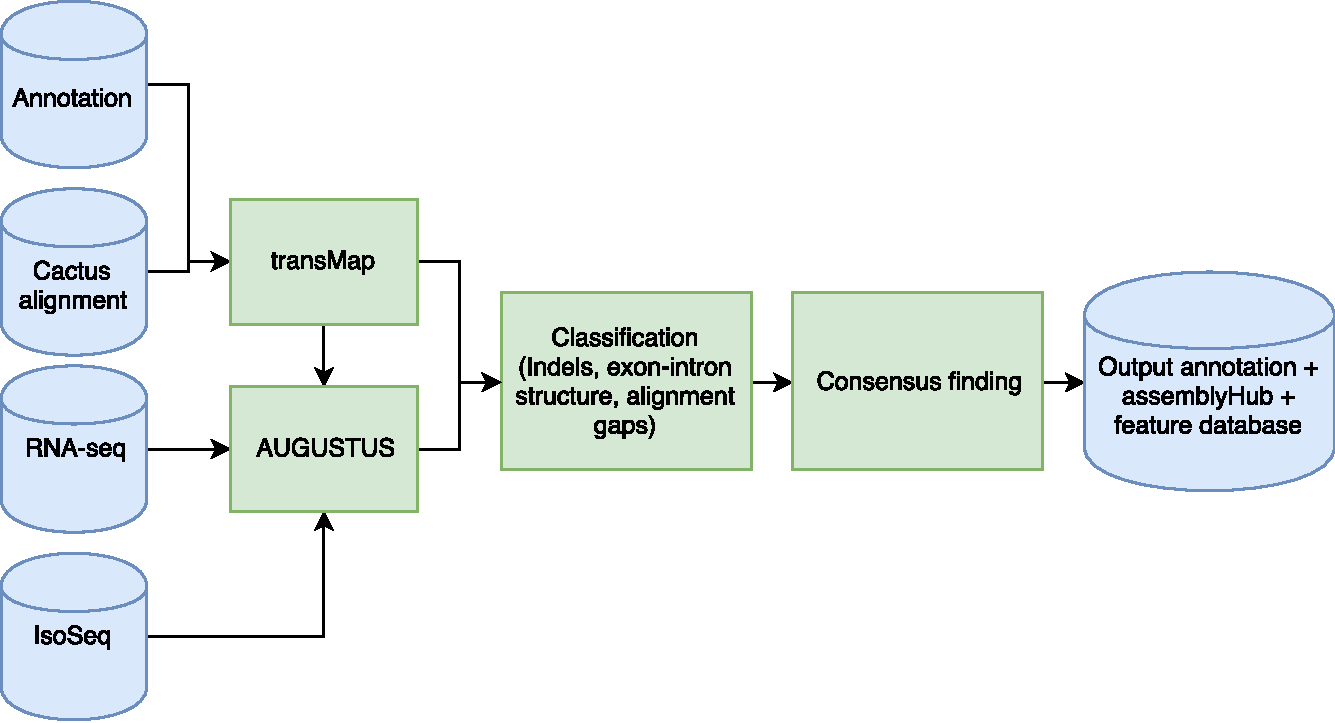
\includegraphics[width=\textwidth,height=\textheight,keepaspectratio]{pipeline_simplified.pdf}
\caption{CAT pipeline schematic}
The CAT pipeline takes as input a HAL alignment file, an existing annotation set and aligned RNA-seq reads. CAT uses the Cactus alignment to project annotations to other genomes using transMap  \citep{stanke2008using}. These transcript projections are then filtered and paralog resolved. Optionally, AUGUSTUS can be run into up to four parameterizations. All transcripts are classified for extrinsic support and structure and a ‘chooser’ algorithm picks the best representative for each input transcript, incorporating \textit{ab-initio} transcripts when they provide novel supported information. The final consensus gene set as well as associated feature tracks are used to create a assembly hub ready to be loaded by the UCSC Genome Browser. See Supplementary Figure \ref{supp_fig:pipeline} and Supplementary Note 1 for more detail.
\label{fig:pipeline}
\end{figure}

\subsection*{Annotation of great apes}

The previous generation of great ape assemblies (panTro4, ponAbe2 and gorGor4) as well as the new SMRT (PacBio) great ape assemblies (\citealt{gordon2016long}, Kronenberg et al., submitted) were annotated by CAT, using GRCh38 and GENCODE V27 as the reference. On average, CAT identified 141,477 more transcripts and 25,090 more genes in the new SMRT assemblies of the great apes compared to the Ensembl V91 annotation of the previous generation of great ape assemblies. Relative to the existing human annotation, the CAT annotations represent an average of 95.0\% of GENCODE gene models and 94.3\% of GENCODE isoforms in the SMRT great ape assemblies. This increase in isoform representation is mostly due to the large number of isoforms annotated by GENCODE and reproduced in these genomes, while the increase in gene content is due to the mapping over of non-coding genes poorly represented in the Ensembl annotation. Comparing the CAT annotations of SMRT great apes and older assemblies, we see an average increase of 610 genes (1.9\%) and 3,743 isoforms (1.0\%) (Supplemental Figure \ref{supp_fig:primate_completeness}) in the SMRT assemblies; given this relatively small increase, most of the observed increase in genes and isoforms in the CAT annotations relative to the Ensembl annotations are therefore a result of the CAT annotation process rather than the updated assemblies.

Conversely to the overall increases in genes and isoforms, CAT identifies on average 3,553 fewer protein-coding genes than Ensembl. However, this brings the total number of coding genes more closely in line with the GENCODE annotation of human, as Ensembl has an average of 2,081 more protein-coding genes in great apes than GENCODE has for human (Supplemental Figure \ref{supp_fig:primate_completeness}). 

To evaluate these annotations in a non-species-biased fashion, consensus isoform sequences created from Iso-Seq reads for each species were compared to their respective species annotations. As a baseline comparison, equivalent human data was compared to the high-quality human GENCODE V27 annotation. The CAT annotation of both the SMRT and older great ape assemblies (which used the raw Iso-Seq reads during the annotation process) and the Ensembl annotation of the older assemblies were compared. We calculated the rate of isoform concordance, that is the fraction of consensus Iso-Seq sequences that match either exactly or fuzzily an annotated isoform (Figure \ref{fig:primate}A; methods). Fuzzy matching allows for the intron boundaries to shift slightly in a isoform. For the SMRT chimpanzee (74.0\%/82.1\% exact/fuzzy matching) and orangutan (71.4\%/80.4\%) genome assemblies the isoform concordance rates were comparable to the rate for human (74.6\%/82.1\%). The gorilla GSMRT3.2 assembly showed lower concordance (67.6\%/76.9\%), likely due to the higher indel error rate in that assembly (Supplemental Figure \ref{supp_fig:primate_indels}). In contrast, the isoform concordance rate for the older assemblies was lower (on average 60.0\%/69.6\%), mostly reflecting exons in gaps and mis-joins, and was lower still for the existing Ensembl annotations (on average 47.9\%/57.6\%).


\begin{figure}
\centering
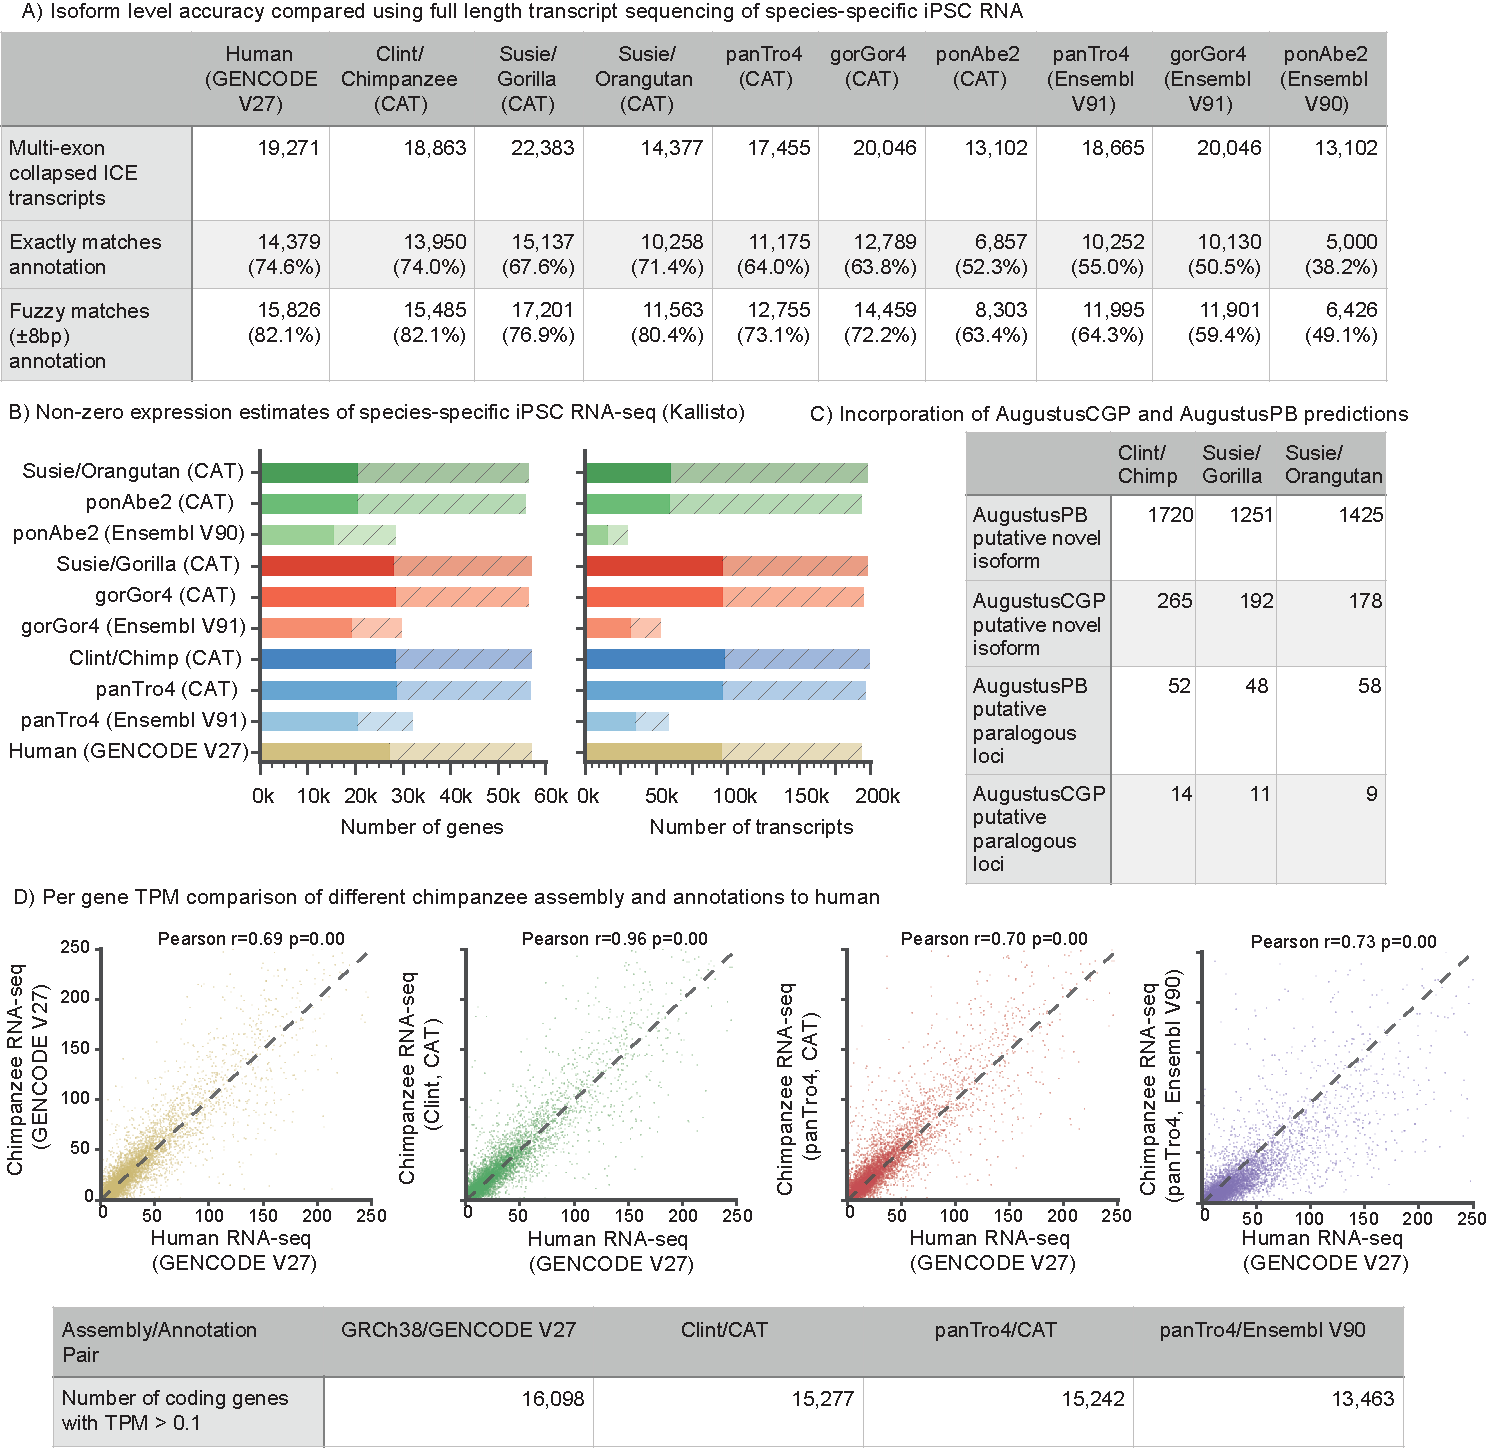
\includegraphics[width=0.8\textwidth,height=0.8\textheight,keepaspectratio]{figure2-primate_v10.pdf}
\caption{Primate annotation}
A) Validating CAT annotations using Iso-Seq data. As a baseline comparison, Iso-Seq data from human iPSCs were compared to the GENCODE V27 annotation. Iso-Seq data from chimpanzee, gorilla and orangutan iPSC lines were compared to respective species-specific annotations. The Iso-Seq data were clustered with ICE and collapsed using ToFU \citep{gordon2015widespread}. CAT annotation of PacBio great apes showed similar isoform concordance to human, and improvement over the older assemblies. B) Kallisto \citep{bray2015near} was used to quantify liver Illumina RNA-seq from each species on both the gene and transcript level on the existing and new great ape assemblies. Solid bars are transcripts or genes with transcripts per million (TPM) \textgreater 0.1, while shaded hatched bars are the remainder of the annotation sets. CAT annotation of great apes shows nearly the same number of expressed genes and isoforms as the GENCODE reference on human with the exception of orangutan. C) The number of novel isoforms and paralogous genes with Iso-Seq support discovered by analysis of AugustusPB and AugustusCGP predictions for each species. D) Kallisto protein-coding gene-level expression for chimpanzee iPSC RNA-seq is compared to human across all of the chimpanzee annotation and assembly combinations as well as when mapped directly to human. In all cases the x-axis is the TPM of human iPSC data mapped to human. The highest correlation (Pearson r=0.96) is seen when comparing Clint annotated with CAT to GRCh38 annotated with GENCODE V27.
\label{fig:primate}
\end{figure}


To assess the utility of CAT annotations for short-read analysis of RNA expression, species-specific induced pluripontent stem cell (iPSC) Illumina RNA-seq data were quantified (Figure \ref{fig:primate}B). Comparing the annotations of the older assemblies, CAT identified an average of 9,518 more genes and 54,107 more transcripts with measurable expression compared to Ensembl.

We might expect the per-gene abundance estimates of the majority of genes in matched cell types to agree between species, particularly for closely related species. It is reasonable to therefore prefer \textit{a priori} an annotation of the great apes that produces expression estimates that agree with expression estimates from the matched human data using the GENCODE annotation. Doing these comparisons, we find better correlations on average using the CAT annotation of the older assemblies (avg. Pearson r=0.63; Figure \ref{fig:primate}D, Supplemental Figure \ref{supp_fig:primate_expression}) than the Ensembl annotations of the older assemblies (avg. Pearson r=0.44). However, we find by far the highest correlation when CAT annotates the SMRT primate assemblies (avg. Pearson r=0.90). This reflects the increased representation in the updated assemblies of transcript sequence, especially 3` UTRs that are important for quantifying poly(A) primed RNA-seq (Kronenberg et al., submitted). Notably, we find that the correlations between the CAT annotations of the SMRT assemblies and the matched human data are higher than when mapping the species-specific data back to the human GENCODE annotations and comparing to the human data (Figure \ref{fig:primate}D, Supplemental Figure \ref{supp_fig:primate_expression}), demonstrating the benefit of having species-specific annotations within closely related species that have clear cross-species orthology relationships. Analysis at the isoform level showed the same patterns (Supplemental Figure \ref{supp_fig:primate_transcript_expression}), albeit with slightly weaker correlations.

Predictions performed by AugustusCGP and AugustusPB were incorporated into the gene sets based on the presence of splice junctions supported by RNA-seq or Iso-Seq and not present in the transMap/AugustusTMR-derived annotations (Figure \ref{fig:primate}C). An average of 1,677 novel isoforms and 64 novel loci were found across the assemblies with at least one Iso-Seq read supporting the prediction.

CAT provides new metrics for diagnosing assembly quality. In the process of annotating the great ape genomes, we noticed that assemblies that had undergone Quiver and Pilon  \citep{walker2014pilon} correction still exhibited a systematic bias towards coding deletions. These were identified to be related to heterozygosity in the input dataset and a variant-calling-based correction method (Kronenberg et al., submitted) was developed to resolve these issues, dramatically lowering the coding indel rate and reducing systematic bias (Supplemental Figure \ref{supp_fig:primate_indels}). CAT can also measure gene assembly contiguity by reporting the number of genes whose transcripts end up split across multiple contigs, or on disjoint intervals in the same contig. Comparison of split gene metrics between the old and new primate assemblies shows 504 fewer split genes in chimpanzee, 560 fewer in gorilla and 1,858 fewer in orangutan (Supplemental Figure \ref{supp_fig:primate_split_genes}).


\subsection*{Annotation of personal human diploid assemblies}

High-quality \textit{de novo} assembly of a human genome is increasingly feasible; both Pacific Biosciences  \citep{chin2016phased,huddleston2016discovery,korlach2017novo} (Falcon) and 10x Genomics  \citep{weisenfeld2017direct} (Supernova) provide tools to construct phased, diploid assemblies. Annotating diploid assemblies provides a window into haplotype-specific structural variation that may affect gene expression. To evaluate the ability of CAT to provide this analysis, Progressive Cactus alignments were generated between hg38 and the two haploid cell line assemblies, CHM1 (GCA\_001297185.1) and CHM13 (GCA\_000983455.2) as well as the 10x Genomics diploid assemblies of four individuals (NA12878, NA24385, HG00512 and NA19240).

An average of 98.5\% of genes present in GENCODE V27 were identified in CHM1/CHM13, while an average of 97.3\% of genes were identified in the 10x Supernova assemblies. (Figure \ref{fig:human_metrics}A). After filtering, an average of 552 genes in the PacBio assemblies and 461 genes in the 10x assemblies had frame-shifting indels (Figure \ref{fig:human_metrics}B). Compared to ExAC, which found between 75 and 125 putative truncating events per individual  \citep{karczewski2016exac}, this result suggests indel errors in the assemblies are producing false positives. All assemblies exhibit systematic overrepresentation of deletions, including the Pacbio assemblies despite coming from haploid cell lines (Figure \ref{fig:human_metrics}B). Split gene analysis found the CHM1 assembly to be the most gene contiguous, with only 39 genes split across multiple contigs, and the PacBio assemblies overall more contiguous (Figure \ref{fig:human_metrics}C). Gene contiguity is measured by looking at genes with multiple alignments post paralog resolution that start and end nearby in transcript coordinates.

Manual analysis of genes with different transMap coverage in CHM13 relative to CHM1 led to the discovery of the example region in Figure \ref{fig:human_example}A. This deletion removes most of the exons of \textit{TRIB3}, a pseudokinase associated with type 2 diabetes  \citep{shi2009association} (Supplemental Figure \ref{supp_fig:trib3}). Similar analysis in the diploid assembly of NA12878 led to the discovery of a tandem duplication involving an exon of TAOK3 in one haplotype (Figure \ref{fig:human_example}B).

\begin{figure}
\centering
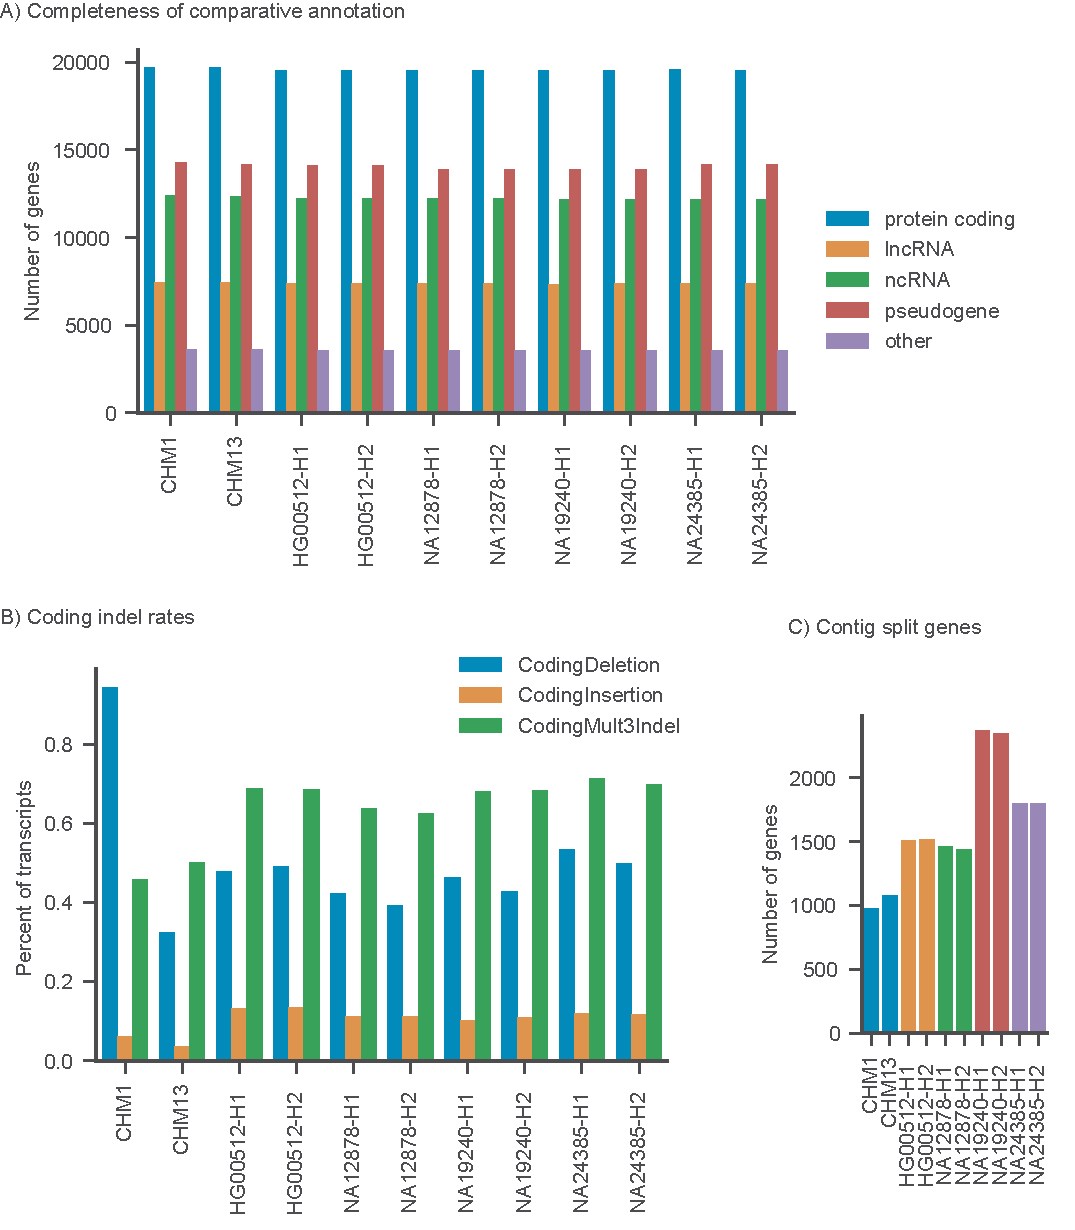
\includegraphics[width=\textwidth,height=0.75\textheight,keepaspectratio]{human-metrics.pdf}
\caption{Pseudo-diploid human annotation metrics}
A) The number and fraction of genes comparatively annotated from GENCODE V27 in each assembly. GENCODE biotypes are simplified into protein coding, lncRNA, ncRNA, pseudogene and other. Other includes processed transcripts, nonsense-mediated decay, and immune-related genes. B) Frame-shifting insertions, deletions and multiple of 3 indels that do not shift frame are reported for each assembly. Consistent with the great ape genomes, there is a systematic over-representation of coding deletions in Falcon assemblies, despite these assemblies coming from haploid cell lines. 10x Supernova assemblies also exhibit similar properties. C) Split gene analysis reports how often paralog-resolved transcript projections end up on different contigs, which can measure assembly gene-level contiguity. PacBio assemblies, especially CHM1, are the most contiguous.
\label{fig:human_metrics}
\end{figure}

\begin{figure}
\centering
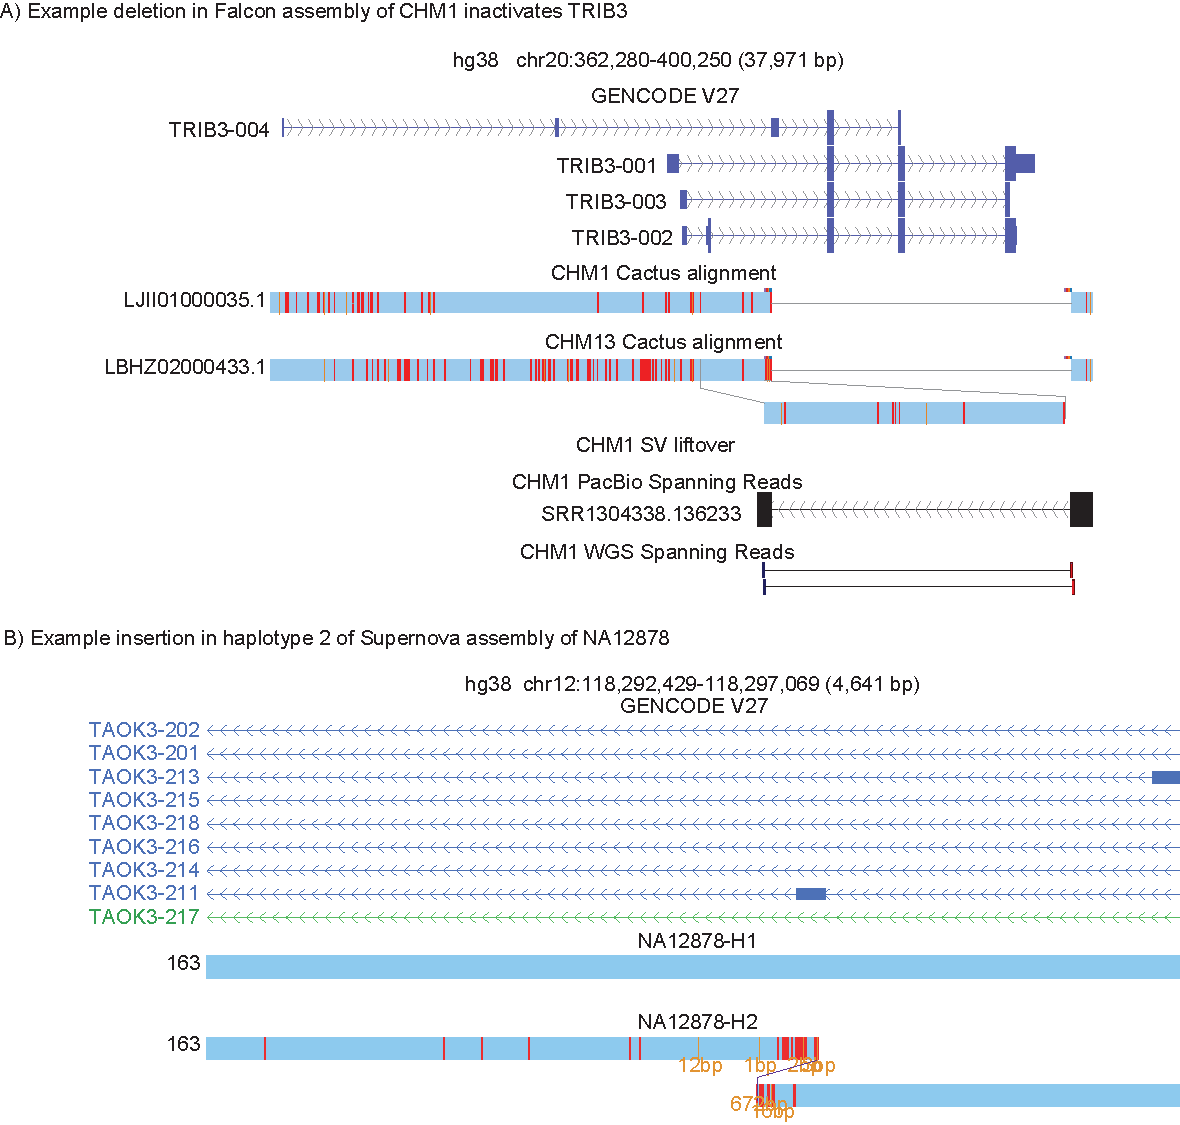
\includegraphics[width=\textwidth,height=0.75\textheight,keepaspectratio]{human-examples.pdf}
\caption{Pseudo-diploid human annotation examples}
A) UCSC Assembly Hub \citep{nguyen2014comparative} showing \textit{TRIB3} deletion in CHM1. Analysis of genes found in one genome and not the other led to the discovery of a novel structural variant specific to CHM1, which disables the gene \textit{TRIB3}. Spanning reads were found in both PacBio and Illumina whole-genome sequencing that validate the deletion. B) An example insertion near an exon of \textit{TAOK3} seen in one haplotype of NA12878. It was not possible to determine if this insertion effected transcription of this gene.
\label{fig:human_example}
\end{figure}

\subsection*{Reannotating the rat genome}

We tested CAT's ability to reannotate the rat genome using information from the mouse genome. These genomes differ by approximately 0.18 substitutions/site, much more, for example, than the 0.04 substitutions/site separating the human and orangutan genomes \citep{karolchik2003ucsc}.

CAT was run on a Cactus alignment between mouse (mm10) and rat (rn6) using rabbit (oryCun2), Egyptian jerboa (jacJac1) and human (hg38) as outgroups. To provide hints to AUGUSTUS, RNA-seq data were obtained from SRA  \citep{fushan2015gene,cortez2014origins,liu2016identification} (Supplemental Table \ref{supp_table:rnaseq_sra_table}). For comparison we used existing Ensembl and RefSeq rat annotations and ran the MAKER2 pipeline  \citep{cantarel2008maker} to generate an annotation set. MAKER was provided both a Trinity  \citep{haas2013novo} \textit{de novo} assembly of the input RNA-seq data provided to CAT (MAKER does not process raw RNA-seq) as well as the mouse protein sequences from GENCODE VM11, together providing a comparable input set to what CAT had. 
  
CAT comparatively annotated 78.1\% of genes and 91.9\% of protein-coding genes present in GENCODE VM11 on rn6 (Supplemental Figure \ref{supp_fig:rat_completeness}), representing an increase of 14,675 genes and 74,308 transcripts over Ensembl V90, 5,104 genes and 32,157 transcripts over RefSeq and 14,541 genes and 81,022 transcripts over Maker. 13,651 loci were identified with no overlap to any other annotation set (Supplemental Figure \ref{supp_fig:rat_locus_venn}).

We compared CDS exon and CDS intron predictions between annotation sets (Table \ref{table:rat_similarity}A, Supplemental Figure \ref{supp_fig:rat_exon_intron}). We measured precision and recall of coding intron and exon intervals based on comparing the CAT annotation to EnsemblV90, where precision is the proportion of CAT exons/introns that exactly match Ensembl, and recall is the proportion of CAT exons/introns that exactly match Ensembl over the number of exons/introns CAT annotated. Ensembl, RefSeq and CAT CDS exon annotations were all comparably similar (between 0.648 and 0.659 Jaccard similarity), while for CDS introns CAT and RefSeq displayed the highest Jaccard similarity (0.841). In all comparisons MAKER was the outlier (Table \ref{table:rat_similarity}B) with the lowest similarity to the other sets.
  
The input RNA-seq dataset was used for isoform quantification against the CAT, MAKER, Ensembl and RefSeq transcriptomes (Figure \ref{fig:rat_validation}A). CAT identified 1,881 protein-coding genes and 1,011 lncRNAs with measurable expression not present in either Ensembl or RefSeq. CAT also identified 27,712 expressed coding splice junctions not in the union of RefSeq and Ensembl, for a total of 21,267 novel expressed isoforms. 5,526 of the 13,651 loci unique to CAT had measurable expression. 

AugustusTMR, which uses transMap and RNA-seq, provides CAT with a way to improve transcript predictions projected between species. Comparing the 10,335 multi-exon protein-coding transcripts in which the AugustusTMR prediction differed from the input transMap projection, we see considerable overall improvement in resulting RNA-seq support of predicted splice boundaries in the AugustusTMR transcripts (Figure \ref{fig:rat_validation}B). 

\subsection*{Annotation of a diverse set of mammals}

Finally, to test CAT's ability to annotate across a substantial and diverse range of genomes, 13 mammalian genomes were comparatively annotated using the mouse (mm10) GENCODE VM15 as the reference transcript set (Figure \ref{fig:13way}A). Species-specific RNA-seq was used for every genome (Supplemental Table \ref{supp_table:rnaseq_sra_table}). To assess the completeness of these annotation sets, 4,104 benchmarking universal single-copy orthologs (BUSCO) were used  \citep{simao2015busco}, which by design should be nearly uniformly present in each of these genomes. On average, only 108 BUSCO genes (2.63\%) were not annotated by CAT in each genome (Supplementary Table \ref{supp_table:busco}). 


\begin{figure}
\centering
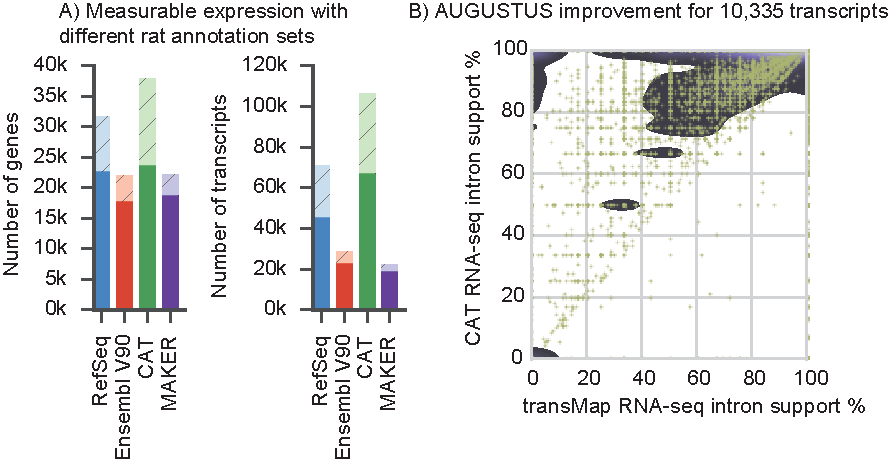
\includegraphics[width=\textwidth,height=\textheight,keepaspectratio]{figure5-rat_v18.pdf}
\caption{Validation of CAT annotation using rat}
A) Each transcript set was used to construct a Kallisto  \citep{bray2015near} index, and then all of the input RNA-seq for annotation were quantified. Solid bars are genes or transcripts with non-zero expression (TPM\textgreater 0.1) estimates, while light hatched bars are the remainder of the annotation set. CAT provides an annotation set with slightly more detectable genes than other annotation methods, and far more detectable isoforms. B) AugustusTMR provides a mechanism to clean up transcript projections and shift splice sites, fixing alignment errors as well as real evolutionary changes. Most of the 10,335 AugustusTMR transcripts chosen in consensus finding show an improvement in RNA-seq support, which is one of the features used in consensus finding.
\label{fig:rat_validation}
\end{figure}

\begin{table}
\centering
A) Precision and recall in CAT annotation of rat\\
\begin{tabular}{|c|c|c|c|c|} \hline
Annotation & Exon precision & Exon recall & Intron precision & Intron recall \\ \hline
CAT & 0.703 & 0.559 & 0.861 & 0.734 \\ \hline
MAKER & 0.507 & 0.582 & 0.610 & 0.746 \\ \hline
\end{tabular}

\vspace{5mm}
B) Jaccard Similarity in rat annotation sets \\
\begin{tabular}{|c|c|c|} \hline
Annotation pair & Exon Jaccard similarity & Intron Jaccard similarity \\ \hline
EnsemblV90/RefSeq & 0.658 & 0.749 \\ \hline
CAT/EnsemblV90 & 0.649 & 0.740 \\ \hline
CAT/RefSeq & 0.648 & 0.841 \\ \hline
EnsemblV90/MAKER & 0.514 & 0.364 \\ \hline
CAT/MAKER & 0.484 & 0.334 \\ \hline
MAKER/RefSeq & 0.464 & 0.337 \\ \hline
\end{tabular}
\caption{Rat annotation similarity metrics}
A) Precision is the number of coding exons or coding introns that exactly match divided by the number of exons or introns in the Ensembl annotation, while recall is the number that exactly match divided by the number of exons or introns in the CAT or, respectively, MAKER annotation. B) Jaccard similarity of CDS introns and exons between rat annotation sets shows high similarity between CAT and existing Ensembl and RefSeq annotations, comparable to the similarity between Ensembl and RefSeq themselves.
\label{table:rat_similarity}
\end{table}

\begin{figure}
\centering
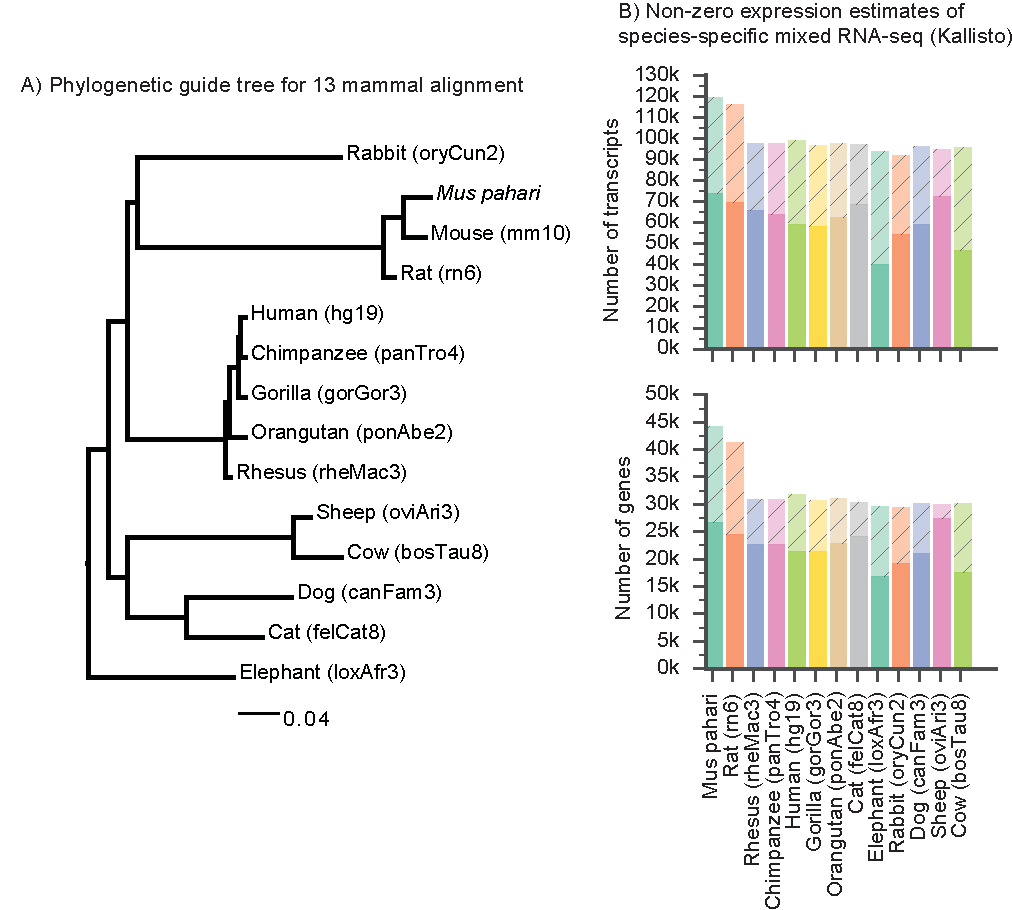
\includegraphics[width=0.7\textwidth,height=0.7\textheight,keepaspectratio]{13way-v5.pdf}
\caption{13-way annotation}
A) The phylogenetic guide tree for the 14-way mammal alignment. See the methods section for the exact Newick format tree. B) The gene annotation sets for each of the 13 mammalian genomes were quantified against the mixed input RNA-seq sets obtained from SRA. Genes or transcripts with TPM\textgreater 0.1 are solid colors, while genes or transcripts with no measurable expression are shaded. An average of 2.8 isoforms per gene per genome had quantifiable expression, suggesting that CAT can infer isoform information across long branch lengths.
\label{fig:13way}
\end{figure}

\begin{table}
\centering
\begin{tabular}{|c|c|c|c|c|c|} \hline
Exon precision & Exon recall & Intron precision & Intron recall & Isoform precision & Isoform recall \\ \hline
0.532 & 0.688 & 0.777 & 0.912 & 0.408 & 0.752 \\ \hline
\end{tabular}
\vspace{5mm}

\caption{Precision and recall of CAT annotation of hg19 using mouse isoforms}
Precision and recall are measured by looking at exact matches of coding introns, exons and isoforms. Isoforms are compared on a coding intron chain level. Precision and recall are defined in the same way as in Table \ref{table:rat_similarity}.
\label{table:validation}
\end{table}

To estimate the usefulness of these annotation sets, the input RNA-seq datasets were used to quantify expression of the annotation sets (Figure \ref{fig:13way}B). The main factor in measurable expression is the variety of the input RNA-seq datasets, as exemplified by the ability to measure expression of 88.9\% of genes annotated in the sheep genome. 

To assess the CAT translation of annotations over large phylogenetic distances, as well as provide a baseline validation of CAT performance, the annotation of human hg19 (GRCh37) produced in the representative mammalian genome annotation was compared to the current human GENCODE annotation set for that assembly (GENCODE V27lift37). Of the 19,233 ICE isoforms detected when running ToFU  \citep{gordon2015widespread} against hg19, 12,911 (67.2\%) fuzzy matched a CAT isoform compared to 15,920 (82.8\%) of the human GENCODE annotations. Precision and recall analysis shows results similar to the rat annotation, with better matches in introns. 91.2\% of CAT introns and 75.2\% of CAT protein coding isoforms match GENCODE (Table \ref{table:validation}).

\section*{Discussion}

% Need statement
Gene annotation is a longstanding and critical task in genome informatics that must now be scaled to handle the rapidly increasing number of available genomes. At the time of writing there were 570 vertebrate genomes available from NCBI, but only 100 (17.5\%) and 237 (41.6\%) had Ensembl and RefSeq annotations, respectively.

% Innovations
We introduce CAT to help meet this need, building around a number of key innovations. 
% Better alignment
Firstly, CAT utilizes the reference-free, duplication-aware multiple genome alignments we have developed. This allows CAT to annotate multiple genomes symmetrically and simultaneously, breaking from the traditional pattern of annotating each new genome individually, as is currently the practice for the RefSeq, Ensembl and MAKER gene-building pipelines.
% Orthology relationships
Not only does this solve a key scalability issue 
by annotating multiple genomes simultaneously and consistently, CAT is able to produce orthology mappings, naming each equivalence class of orthologs based upon an initial reference annotation, and add to this sets of newly discovered genes. This can provide valuable evolutionary insights. For example, the analysis of the rat genome shows that many of the alternative isoforms and projected transcription start sites identified by GENCODE in mouse genes are supported by expression analysis in rat (Supplemental Figure \ref{supp_fig:unsupported_junctions}).

% Leveraging existing annotations
A second key innovation made by CAT is its leveraging of existing reference annotations. A huge amount of effort has been placed into the annotation of key species, such as human and mouse, employing a myriad of technologies and extensive, labor-intensive manual curation. It is very unlikely that this effort will be replicated across a significant fraction of other genomes, so instead we propose the `project and augment' strategy employed by CAT to annotate related genomes. Here we show that this strategy is very clearly able to improve the annotation of great ape genomes, using the human GENCODE set as the reference, and we make the case that we can even improve the annotation of a genome as well studied as the rat. 

% Extrinsic information, inc. long reads. for unbiased genome annotation
To circumvent the reference bias of existing annotations and to discover new genes and isoforms, CAT is able to integrate multiple forms of extrinsic information, using multiple, novel parameterizations of the AUGUSTUS algorithms. This includes use of new long-read RNA data, in particular Iso-Seq data, and shortly will integrate nanopore-based long-read data \citep{byrne2017nanopore}. Using this expression data not only allowed us to confirm expression of a substantial fraction of isoforms but allowed us to discover thousands of novel isoforms and dozens of novel genes in the great ape genomes.

% Diploid, personal annotation
With the advent of more affordable \textit{de novo} genome assembly, there is renewed interest in the generation of \textit{de novo} human genomes, and in general the creation of multiple \textit{de novo} genomes for a species. This has the advantage of providing fully independent reconstruction and is particularly appropriate for sequences that are highly divergent from the reference, e.g. structural variations. However, such assemblies do not negate the need for genome comparison; Cactus can be parameterized to rapidly create sensitive whole-genome alignments of human genomes, and here we have demonstrated that CAT can be used to build upon this to produce a high-quality diploid gene annotation and ortholog mapping. 

% Practical considerations for future projects
CAT works best when provided RNA-seq data, but for many species this may not be possible. From our experience, a reasonable amount (on the order of 50 million reads) of RNA-seq from tissues like brain and liver is fairly informative. Using poly(A)-selected libraries is recommended, as it greatly reduces false positive predictions in AugustusCGP. Iso-Seq data allowed for the discovery of thousands of novel isoforms in the great apes but may be too expensive for many projects. In clade genomics projects, we would suggest generating RNA-seq for a few of the species and then reliance on the coordinate mapping that AugustusCGP and homGeneMapping provide to evaluate support in other members of the clade. 

% Practical / engineering considerations
A key barrier to the use of bioinformatics tools is their ease of use; we have focused on providing cloud agnostic distributions of the CAT software so that, despite its complexity, it can be run within a uniform computational environment by external groups. 

% Future development
CAT is not without limitations. In the future it would be good to use the genome alignments to not only project transcripts, but to use the evolutionary conservation signatures to predict the potential likelihood of projected annotations being coded  \citep{lin2011phylocsf}. CAT also does not yet provide means to detect new processed, unprocessed and unitary pseudogene predictions other than via projection of existing annotations. CAT’s current implementation also does not attempt to put weights on the features used for constructing a consensus gene set. Instead, it simply scores transcripts based on the sum of all features evaluated. In the future deep learning methods could be added to CAT to construct feature weights and improve consensus finding, better mimicking the labor intensive efforts of manual annotators who currently weigh such evidence. 

% Future application
An earlier version of CAT was used to annotate the PacBio-based assembly of the gorilla genome  \citep{gordon2016long} as well as produce the current Ensembl annotations for 16 laboratory mouse strains as part of the Mouse Genomes Project \citep{lilue2018multiple} (\url{http://www.sanger.ac.uk/science/data/mouse-genomes-project}). In addition, CAT has been proposed for the Vertebrate Genomes Project (VGP), which aims as a pilot project to assemble and annotate one member of every order of vertebrate species. CAT also will be used on the 200 Mammals Project, which aims to add approximately 140 new mammalian genome assemblies to the existing set (\url{https://karlssonlab.org/2017/08/03/the-200-mammals-project/}). These projects will provide a new understanding of gene evolution.

\section*{Materials and Methods}

CAT produces as output a series of diagnostic plots, an annotation set for each target genome, and a UCSC comparative assembly hub  \citep{nguyen2014comparative}. Both the pipeline and associated documentation can be found at \url{https://github.com/ComparativeGenomicsToolkit/Comparative-Annotation-Toolkit}. CAT is constructed using the Luigi (\url{https://github.com/spotify/luigi}) workflow manager, with Toil  \citep{vivian2017toil} used for computationally intensive steps that work best when submitted to a compute cluster. 

\subsection*{RNA-seq}

CAT annotation is improved when species-specific RNA-seq data are provided. These data are used as hints for AugustusTMR and AugustusCGP. In AugustusTMR, RNA-seq helps fill in missing information in the alignment, as well as resolve evolutionary changes. In AugustusCGP, RNA-seq additionally helps prevent false positives inherent in \textit{ab initio} gene finding. For these reasons, RNA-seq was obtained from SRA for all species annotated in this paper. All RNA-seq were aligned to their respective genomes with STAR  \citep{dobin2013star} and the resulting BAM files passed to CAT to construct the extrinsic hints database. See Table \ref{supp_table:rnaseq_sra_table} for accessions and tissue types of RNA-seq data used for annotation. In addition, for the PacBio great ape annotation, RNA-seq data were generated using iPSC lines for human, chimpanzee, gorilla and orangutan derived from cells for the same individuals as the assemblies (Kronenberg et al., submitted). For all expression analyses, Kallisto  \citep{bray2015near} was used.

\subsection*{Annotation set similarity analysis}

Jaccard similarity analysis was performed with BEDTools  \citep{quinlan2010bedtools}. The rat locus overlap analysis was performed with the Kent tool clusterGenes, which requires exonic overlap on the same strand.

\subsection*{Iso-Seq}

Iso-Seq full-length non-chimeric reads (FLNC) were also generated from the great ape iPSC lines and aligned with GMAP  \citep{wu2005gmap}.To perform isoform-level validation in the primates, the Iso-Seq data used as input to CAT were also clustered with isoform-level clustering (ICE) and then collapsed into isoforms using ToFU  \citep{gordon2015widespread}. Ensembl provided a pre-release of their new V91 annotations for panTro4 and gorGor4, but did not yet run their updated pipeline on ponAbe2.

\subsection*{ICE validation}

The output transcripts from ICE were compared to various annotation sets in both an exact and fuzzy matching scheme. In the exact scheme, the genomic order and positions of all of the introns (an intron chain) of a transcript are compared to any ICE isoforms which overlap it. In the fuzzy matching scheme, each annotated intron chain is allowed to move up to 8 bases in either direction and still be called a match.

\subsection*{BUSCO}

The mammalian BUSCO  \citep{simao2015busco} analysis was performed using the mammalia\_odb9 set of 4,104 genes. BUSCO was ran against the complete protein-coding sequence repertoire produced by CAT in that species in the `protein' mode.

\subsection*{Progressive Cactus}

All Cactus alignments except the 14-way mammal alignment were generated using Progressive Cactus (\url{https://github.com/glennhickey/Progressive Cactus}) commit 91d6344. For the mouse-rat alignment, the guide tree was 

\begin{lstlisting}
(((Lesser_Egyptian_jerboa:0.1,(Mouse:0.084509,Rat:0.091589)mouse_rat:0.107923)rodent:0.148738,Rabbit:0.21569)glires:0.015313,Human:0.143908);
\end{lstlisting}

For the primate alignments, the guide tree was 
  
\begin{lstlisting}
(((((((Susie_Gorilla:0.008964,(Human:0.00655,Clint_Chimp:0.00684)human_chimp:0.00122)gorilla_chimp_human:0.009693,Susie_Orangutan:0.01894)great_ape:0.003471,Gibbon:0.02227)great_ape_gibbon:0.01204,Rhesus:0.004991)old_world_monkey:0.02183,Squirrel_monkey:0.01035)monkey:0.05209,Bushbaby:0.1194)primate_anc:0.013494,Mouse:0.084509);
\end{lstlisting}
  
An identical tree (with different assembly names) was used for the alignment of current reference great apes.
  
For the diploid human alignments, the two haploid cell lines (PacBio) or all human haplotypes (10x) were placed under the same node with a very short branch length, with chimpanzee as outgroup. The guide trees were

\begin{lstlisting}
((hg38:0.001,chm1:0.001,chm13:0.001)human:0.01,chimp:0.01);
\end{lstlisting}

and

\begin{lstlisting}
((hg38:0.001,HG00512-H1:.001,HG00512-H2:.001,NA12878-H1:.001,NA12878-H2:.001,NA19240-H1:.001,NA19240-H2:.001,NA24385-H1:.001,NA24385-H2:.001)human:0.01,chimp:0.01);
\end{lstlisting}
  
representing a star phylogeny of the three human assemblies. For the 14-way mammal alignment, the Progressive Cactus commit used was e3c6055 and the guide tree was 
  
\begin{lstlisting}
((((oryCun2:0.21,((Pahari_EiJ:0.03,mm10:0.025107)1:0.02,rn6:0.013)1:0.252)1:0.01,((((hg19:0.00642915,panTro4:0.00638042)1:0.00217637,gorGor3:0.00882142)1:0.00935116,ponAbe2:0.0185056)1:0.00440069,rheMac3:0.007)1:0.1)1:0.02,((oviAri3:0.019,bosTau8:0.0506)1:0.17,(canFam3:0.11,felCat8:0.08)1:0.06)1:0.02)1:0.02,loxAfr3:0.15);
\end{lstlisting}

Slightly out-of-date versions of some assemblies (hg19 and rheMac3) were used because a collaborator had data on those assemblies that they wished to use the alignment to analyze. The rodent and primate subtrees were first aligned separately (the rodent subtree originally included additional mouse strains) \citep{thybert2018repeat,lilue2018multiple}. The two subtrees were then “stitched” together into a single alignment by aligning together their roots along with several Laurasiatheria genomes. This was done to save alignment time by reusing existing alignments.

\subsection*{CAT}

CAT was run on the UCSC Genome Browser compute cluster for all annotation efforts in this publication. CAT commit f89a814 was used. For a detailed description of how CAT works, see both the supplementary text as well as the README.md on GitHub (\url{https://github.com/ComparativeGenomicsToolkit/Comparative-Annotation-Toolkit}). 

\subsection*{Pipeline runtime}

CAT is relatively efficient, taking on the order of thousands of core hours to run. The largest considerations for runtime are running the various parameterizations of AUGUSTUS as well as generating the required cactus alignment. AugustusCGP may run significantly faster on alignments with many genomes by reducing the chunk size from the default, but at the cost of lower quality predictions. AugustusTMR runtime scales linearly with the number of protein-coding transcripts in the input annotation set, but scales non-linearly with the number of extrinsic hints provided, particularly if the hints are contradictory. 

All of the analyses in this paper were run on the UCSC cluster, which uses the cluster management tool Parasol and has 1024 cores with 8GB of RAM per core. CAT was optimized for this, and shouldn't need more memory per core in any case except the AugustusCGP step when the number of aligned genomes exceeds \~10. This can be adjusted by reducing the alignment chunk size that AugustusCGP is given to work with. For example, for the 14-way mammalian analysis, the flags \texttt{--maf-chunksize 1000000 --maf-overlap 200000} were set which kept memory usage under 8GB.

Cactus alignments take on the order of 120 CPU days (2,880 core hours) per internal node on the guide tree, assuming a binary tree. This number can fluctuate by a factor of 2-4 depending on how similar the two genomes being aligned at that node are. Cactus alignments are a mix of high CPU low memory steps with a few high memory steps, with some jobs requiring \~240GB of RAM.

Running CAT on the PacBio primate genomes took a total of 7,030 core hours, with 3,437 of those dedicated to running AugustusTMR, 1,191 dedicated to running AugustusPB, and 2,190 dedicated to running AugustusCGP. Running CAT on the 14-way mammalian alignment took a total of 24,122 core hours, with 14,045 of those dedicated to running AugustusTMR, and 8,225 dedicated to running AugustusCGP.

\section*{Software Availability}
CAT is available on GitHub (\url{https://github.com/ComparativeGenomicsToolkit/Comparative-Annotation-Toolkit}). The exact commit used for these analyses is also in the Supplementary Materials section.

\section*{Acknowledgements}

We would like to thank Brian Raney, Hiram Clawson and the rest of the UCSC Genome Browser team for help creating browser tracks. We would also like to thank James Kent for allowing UCSC Genome Browser compute resources to be used for this project. Finally, we would like to thank Fergal Martin and Paul Flicek for revising the paper and providing a pre-release of the Ensembl V91 annotations on chimpanzee and gorilla, as well as the whole GENCODE consortium for their support and advice. This work was supported, in part, by US National Institutes of Health (NIH) grants U24HG009081 and U41HG007635 to E.E.E., HG007990 to D.H and B.P, and HG007234 to B.P. E.E.E. and D.H. are investigators of the Howard Hughes Medical Institute. (COI: E.E.E. is on the scientific advisory board (SAB) of DNAnexus, Inc.)

\bibliography{references}

\clearpage
\beginsupplement

\section*{Supplementary Note 1}

Below is a walkthrough of the CAT pipeline. Please see the README on github 

(\url{https://github.com/ComparativeGenomicsToolkit/Comparative-Annotation-Toolkit}) 

for the most up-to-date information as well as practical information on how to run the pipeline. 

\subsection*{Whole-genome alignment}
	CAT relies on a reference-free whole-genome alignment produced by the tool Progressive Cactus. One or more of the genomes in the alignment should be a high-quality reference whose existing annotations will be projected. Care should be taken when generating Cactus alignments to provide sufficient outgroup genomes. Having high-quality outgroups improves the resolution of paralogies and rearrangements.

\subsection*{Alignment chaining}
	CAT converts HAL format alignments into pairwise genome alignments via a conversion to the UCSC chain format  \citep{kent2003evolution}. This is accomplished by using the halLiftover tool to provide a PSL-format alignment describing each pairwise relationship to the high-quality reference, and this alignment is then chained via the axtChain tool. 
  
\subsection*{transMap}
	transMap  \citep{stanke2008using,zhu2007comparative} is a process for using pairwise whole-genome alignments to project transcript annotations from one genome to another. The main program in the Kent repository for this process is pslMap. Custom software was written for CAT and included in the Kent repository, including pslMapPostChain which chains together mapped over transcript projection, and transMapPslToGenePred which converts the transcript projections to a gene model, keeping track of frame information and optionally filling in coding and noncoding gaps. Frameshifting gaps are not filled. CAT currently hard-codes those values at 50 bp and 80 bp, respectively.
  
\subsubsection*{transMap filtering, paralogous alignment and gene family collapse resolution}
	After transMap projection, alignments are filtered to their most likely ortholog, and paralogies are detected. This is performed using the tool pslCDnaFilter from the Kent repository using the globalNearBest algorithm. This algorithm scores alignments and returns the set of alignments whose score is within the user-set fraction of the highest score. Setting this value to one ensures that only one alignment is returned, and increasing values allow more alignments to be kept. This value can be tuned by the user based on phylogenetic distance -- larger values increases the rate at which alignments of related genes will be considered paralogous. After this step, coding and non-coding genes are separated and ran through the Kent tool clusterGenes either with or without the -cds flag. This tool clusters genes into loci based on exonic or CDS overlap based on the -cds flag. For each input gene, the highest scoring cluster is found and that gene is assigned to that cluster. Overlapping genes populate the paralogy field. Oppositely, for each cluster identified after paralog resolution, if there is more than one gene associated, it is marked as a gene family collapse (in other words, more than one gene had that cluster as its highest scoring cluster).
    
    Finally, split gene analysis uses the localNearBest algorithm to filter the input alignments. This algorithm allows for sliding window scores across a input transcript, and is designed to filter transcript projections to discontiguous assemblies. If a input transcript has multiple alignments after this filter, and they are immediately adjacent in transcript coordinate space, then this transcript is marked as being split.

\subsection*{AUGUSTUS}
	CAT runs the gene-finding tool AUGUSTUS in up to four distinct parameterizations -- AugustusTM (TM), AugustusTMR (TMR), AugustusCGP (CGP) and AugsutusPB (PB). The output of each of these modes is combined with the original transMap output in the consensus gene set finding process. The first two modes, TM/TMR are intended to reproduce the input isoform exactly, fixing regions where the alignment dropped an exon or introduced a small gap, or where the splice site may have shifted. These modes cannot detect novel genes or transcripts. In contrast, CGP/PB both can detect novel isoforms and genes. However, CGP can only detect one isoform for a locus and cannot find UTRs. CGP also cannot find genes in regions that did not align. 
  
\subsubsection*{AugustusTM/AugustusTMR}
	The primary parameterization of AUGUSTUS for comparative annotation is primarily a method to clean up transMap projections. Due to a combination of assembly error, alignment noise and real biological changes transMap projections have frame-shifting indels, missing or incomplete exons, and invalid splice sites. TM is given every protein-coding transMap projection one at a time with some flanking sequence and asked to construct a transcript that closely matches the intron-exon structure that transMap provides. Since AUGUSTUS enforces a standard gene model, frame shifts and invalid splices will be adjusted to a valid form. In some cases this will mangle the transcript, producing either another isoform or something that does not resemble the source transcript. TMR runs the same inputs to AUGUSTUS, but with less strict weights on the transMap hints such that extrinsic hints from RNA-seq or Iso-Seq have more bearing on the outcome. This is particularly useful in regions where an exon was dropped in the Cactus alignment, or where a rearrangement broke the alignment chains.
  
\subsubsection*{AugustusCGP}
	As TM/TMR is built on the transMap projections, it can neither identify novel genes nor existing genes of the reference annotation for which the mapping entirely failed. For this purpose, AUGUSTUS is run in its new comparative mode (CGP) recently published  \citep{konig2015simultaneous}. This mode uses a novel objective function to simultaneously predict coding transcripts in every genome in a Cactus alignment, taking in extrinsic information from any provided existing annotations as well as RNA-seq and/or Iso-Seq data in any of the aligned genomes. The genome alignment is used to exploit evolutionary content for gene finding (e.g. sequence conservation, conservation of exon boundaries and selective pressure) and to transfer extrinsic evidence across genomes. The latter has the effect that each genome can benefit from the combined evidence for the clade. CGP performs best when high-quality RNA-seq derived from poly(A)-selected libraries is provided for as many genomes as possible. If this is not available, consider providing a FASTA file with previously annotated proteins of one of the currently annotated genomes. 
  
\subsubsection*{AugustusPB}
	PB is run when Iso-Seq data are provided and the appropriate flags set. PB runs AUGUSTUS in single genome \textit{ab initio} + evidence-based gene-finding mode, providing high weight to extrinsic hints derived from Iso-Seq data, and with the model parameterized to allow for alternative isoforms. PB provides the advantage of being able to detect genes in regions that did not align to any of the other genomes.
  
\subsubsection*{Parent gene assignment}
CGP/PB transcripts are then assigned a possible source transcript by comparing their genomic overlap with both filtered and unfiltered transMap projections. If a transcript is assigned to an orthologous projection, then it will be evaluated for being a novel isoform during consensus finding. If a transcript is assigned to a projection that was filtered out during paralog resolution, then it is a candidate being a possible paralog. A likely cause of this situation is a gene family expansion. If a transcript does not overlap with any transMap projections, then it is a candidate novel gene. However, the false positive rate of these is inherently high due to the likelihood of novel genes being dwarfed by the likelihood of assembly or alignment errors leading to no transMap projections in the region.

\subsubsection*{Transcript classification}
	transMap projections are classified by a series of classifiers that evaluate their strength. These classifiers include evaluating whether the projection was complete (100\% coverage), alignment identity, whether the projection ran off the edge of a contig, whether the projection had a 1-1 ortholog relationship, and importantly how many of the exon junctions lie nearby in transcript coordinate space. This original intron classification is very important when assigning isoform relationships. Due to alignment errors and real biological changes, transMap projections may have gaps that are not near the source transcript exon junctions. The number of original introns is an important feature in the consensus finding process, protecting from retroposed pseudogenes as well as isoform switching.
  
	Transcripts produced by TM/TMR are also classified. To do so, they are first aligned in transcript space using BLAT  \citep{kent2002blat}. Alignments are performed twice, once on a whole transcript mRNA level and once using the in-frame CDS sequence using a mode of BLAT that does translation alignment. The mRNA alignments are used to perform the same original intron analysis described above, as well as record standard alignment metrics such as coverage and identity. The CDS alignments are used to evaluate transcripts for having frame-shifting indels. A track of the frame-shifting indels are added to the assembly hubs produced.

\subsubsection*{homGeneMapping}
	homGeneMapping is a tool in the Augustus package for cross-species evaluation of gene sets. It uses Cactus alignments to project the coordinates of genomic features to other genomes. Homologous gene structures are evaluated based on their consistency across species and their agreement with the combined extrinsic evidence for the clade. The latter effectively means, that a gene structure of a species with no native evidence can be "confirmed" with evidence for another species by mapping it through the genome alignment. CAT uses homGeneMapping to evaluate intron and exon features in the target genomes for 1) consistency with the reference annotation and 2) having extrinsic support by the combined RNA-seq and/or Iso-Seq. These measures of support are used in the consensus finding process.

\subsubsection*{Consensus finding}
	The consensus finding process takes in transcripts from every mode and attempts to find the highest quality ortholog for a source transcript. The modes that are capable of predicting new transcripts are also evaluated for providing novel isoforms or novel loci. The final gene set is output with a series of features measuring how confident the prediction is.
  
	To evaluate transMap, TM and TMR transcripts a consensus score is assigned to each. This score is the sum of the alignment identity target alignment coverage, intron/exon annotation support, original intron support, and intron/exon RNA-seq/Iso-Seq support if extrinsic data were provided.
  
	If CGP and/or PB is run, then those transcripts are evaluated for providing novel information. If a prediction did not overlap any transMap projections, then it is tagged as putative novel and incorporated into the gene set. If a prediction overlaps a transMap projection that was filtered out during paralog resolution, then it is tagged as a possible paralog as well as with the names of overlapping transcripts and incorporated into the gene set. If a prediction overlaps a transMap projection and contains a splice junction not seen in the reference annotation, then it is tagged as a novel isoform and incorporated into the gene set as a member of the gene it overlapped with.
  
	After consensus finding is complete, a final filtering process is performed. This filtering process deduplicates and strand resolves the transcript set. Duplicates most often occur when the AUGUSTUS execution modes create an identical transcript model from different input isoforms. In this case, the duplicates are removed and the remaining transcript tagged with the names of alternative source transcripts. Finally, strand resolution throws out transcripts that are on opposite strands. The correct strand is chosen by looking at which contains the most high-quality transcripts.
  
	The consensus finding process provides many user-tunable flags that can be adjusted based on the phylogenetic distances being considered. Users can change how many exons and introns should be supported by the reference annotation and extrinsic sources before being considered. Users can also decide if they want only to consider extrinsic data within that individual species or within all species in the alignment. 

Another consideration is the quality of the input extrinsic data. Low quality RNA-seq data, or RNA-seq libraries not poly(A) selected, lead to a higher false positive rate in CGP. These often manifest as small single exon transcripts that can inflate the rate of putative novel gene calls. Adjusting a cutoff for the number of exons required to be considered novel can help drill down to a set of interesting candidates.

\subsubsection*{Effect of low-contiguity or incomplete assemblies on annotation quality}
Annotating a clade with widely varying assembly quality could potentially impact the quality of the annotation: because CAT uses a multiple alignment to project transcripts, lower-quality assemblies could impact the alignment between high-quality assemblies. However, the aligner we use, Cactus, is careful to mitigate this problem. At each progressive step, it aligns the ingroups against multiple outgroups, preferring assemblies that are marked as high-quality by the user. Any sequence in an ingroup that aligns with an outgroup is guaranteed to be lifted up to be input to the next progressive step, which should ensure that incomplete assemblies, with a lot of missing data, do not drastically affect the alignment between high-quality assemblies. To quantify the effect of low-quality assemblies on Cactus alignments, we compared two alignments: one with human, mouse, and several lower-quality assemblies, including the first drafts of tarsier and tree shrew, which are fairly low-quality, with $<$30kb N50 and are relatively incomplete (high \%N). The guide tree for this alignment was:
\begin{lstlisting}
(((((((hg19:0.00877,gorGor3:0.008964):0.009693,ponAbe2:0.01894):0.015511,rheMac3:0.037601):0.07392,tarSyr1:0.1114):0.034014,tupChi1:0.19114):0.002,(dipOrd1:0.171759,(criGri1:0.14,mm10:0.132282):0.11015):0.114051)euarchontoglires:0.020593,(bosTau7:0.18908,canFam3:0.13303):0.032898);
\end{lstlisting}
where the leaf names refer to the UCSC Genome Browser identifiers for the assemblies. The second alignment was of only the high-quality assemblies human, mouse, rat, and dog, with guide tree:
\begin{lstlisting}
(((mm10:0.0728,rn5:0.0812)mr:0.2603,hg19:0.142):0.0233, canFam3:0.197);
\end{lstlisting}
The coverage of mouse on human in these two alignments was very similar: 31.5\% for the first vs. 31.8\% for the second. We believe this demonstrates that, empirically, the induced alignment between high-quality genomes is unlikely to be drastically affected by the inclusion of low-quality assemblies (though some minor changes are expected), and that the resulting annotations of high-quality assemblies are unlikely to be significantly affected by the presence of low-quality assemblies.

\clearpage

\begin{figure}
\centering
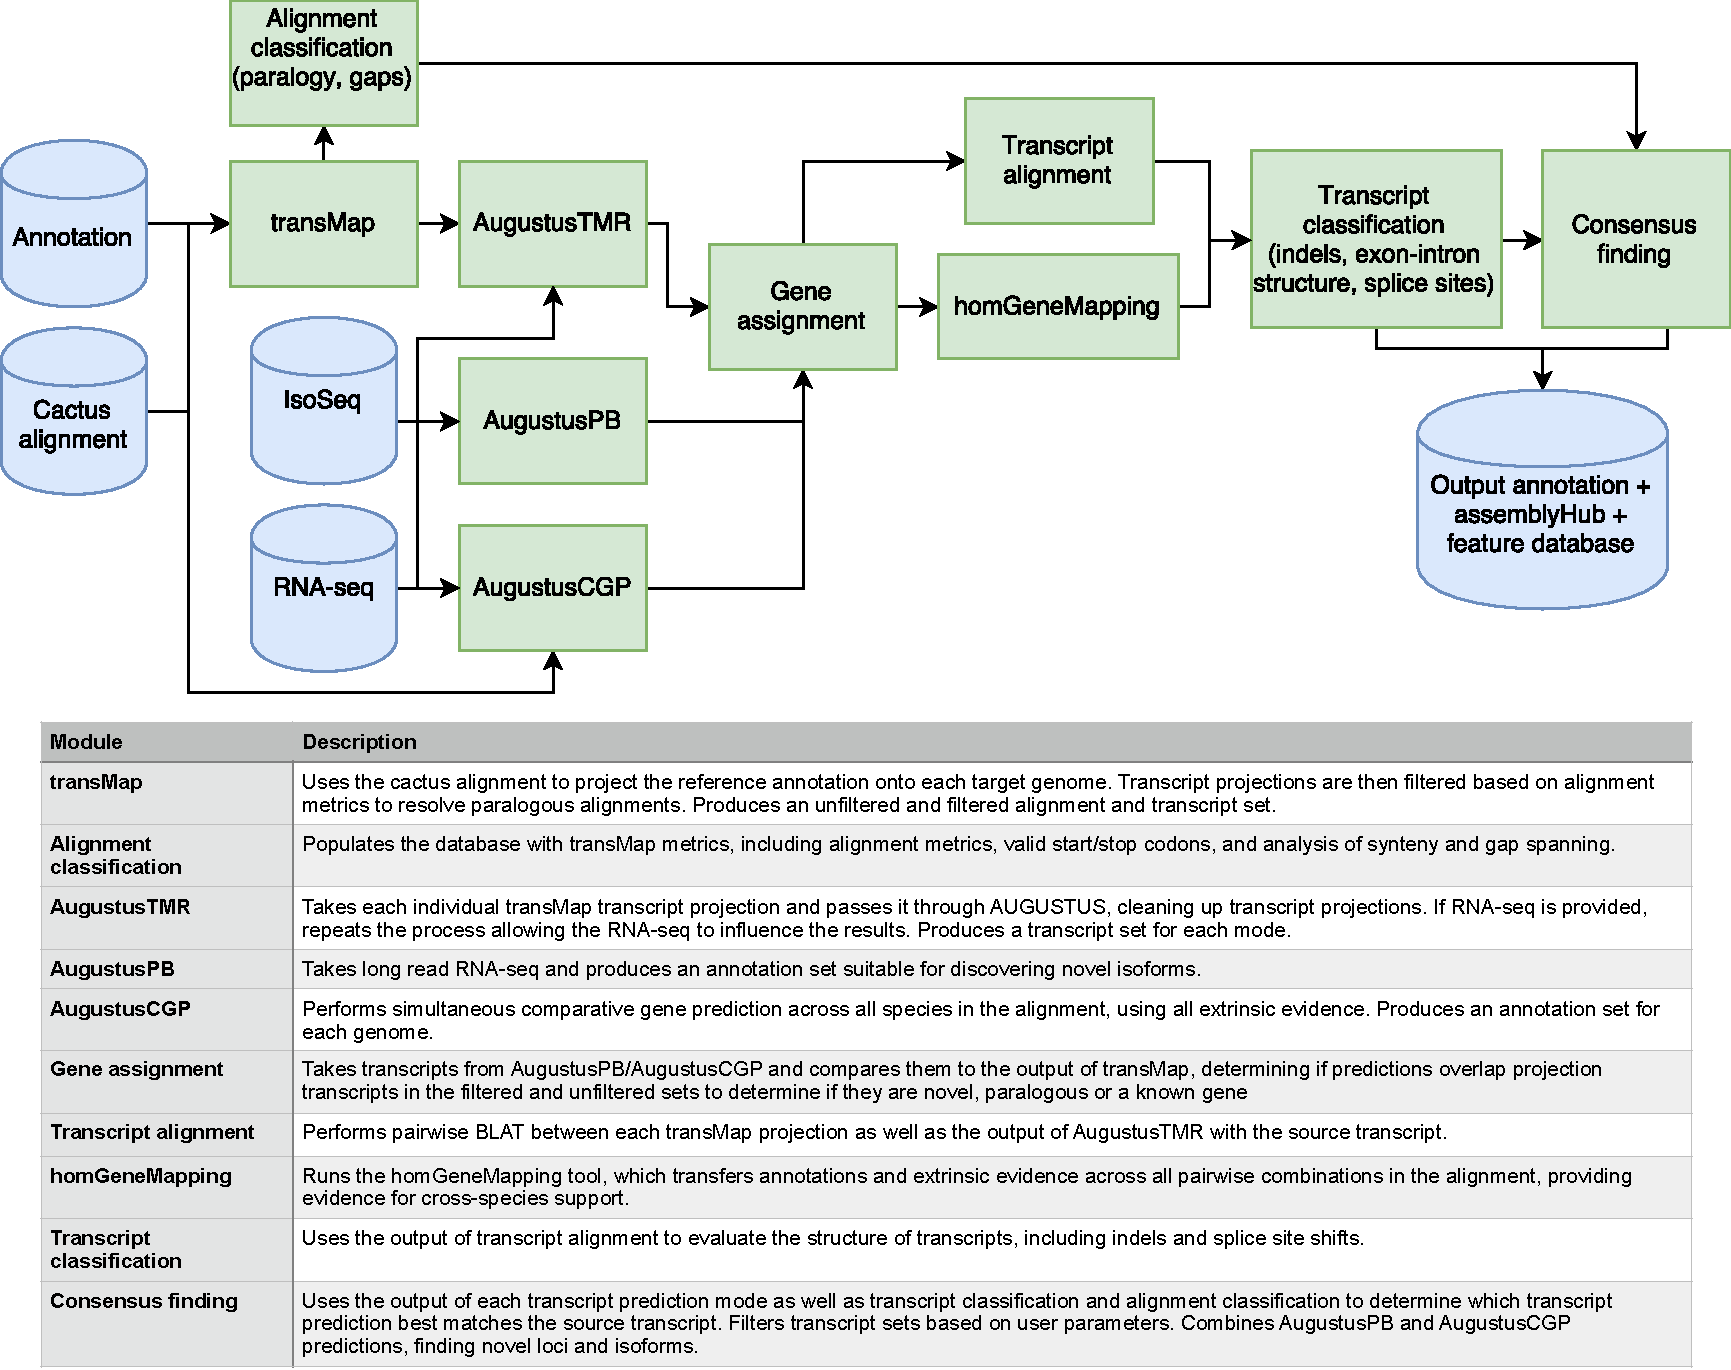
\includegraphics[scale=0.5]{CAT_detailed.pdf}
\caption{CAT detailed pipeline schematic}

\label{supp_fig:pipeline}
\end{figure}

A more detailed schematic of the CAT pipeline. The CAT pipeline takes as input a HAL alignment file, an existing annotation set and aligned RNA-seq reads. CAT uses the Cactus alignment to project annotations to other genomes using transMap  \citep{stanke2008using}. These transcript projections are then filtered and paralog resolved. Optionally, AUGUSTUS can be run into up to four parameterizations. 1) AugustusTMR, treats each transcript projection separately and fixes errors in projection. 2) AugustusPB, uses long-read RNA-seq to look for novel isoforms. 3) AugustusCGP  \citep{konig2015simultaneous} uses the Cactus alignment to simultaneously predict protein-coding genes in all aligned genomes. CGP and PB predictions are assigned to transMap projections where possible based on overlap. All transcripts are classified for extrinsic support and structure and a ‘chooser’ algorithm picks the best representative for each input transcript, incorporating CGP and PB transcripts when they provide novel supported information. The final consensus gene set as well as associated feature tracks are used to create a assembly hub ready to be loaded by the UCSC Genome Browser. The table below the schematic gives a brief overview of each module and the outputs it produces.

\begin{figure}
\centering

A)

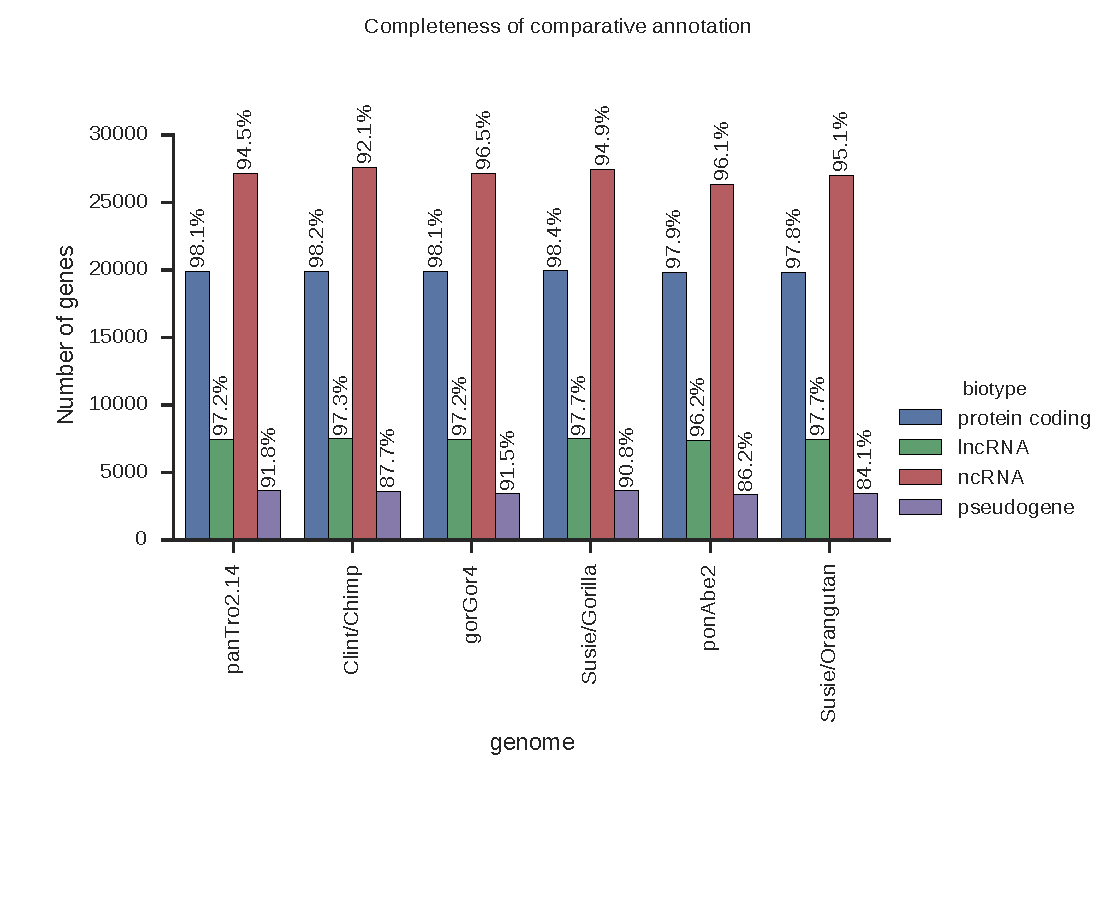
\includegraphics[scale=0.7]{primate_completeness_old_and_new.pdf}

B)

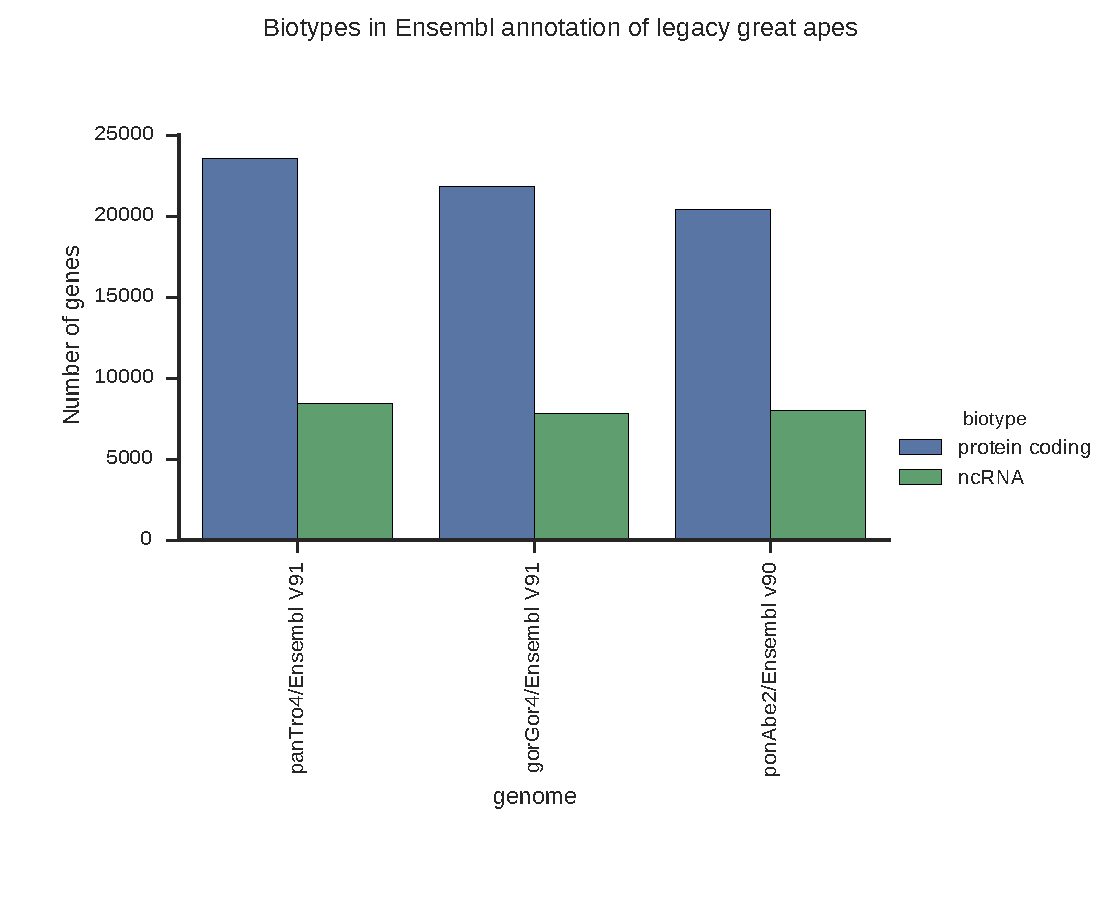
\includegraphics[scale=0.5]{ensembl_primate_biotypes.pdf}

\caption{Primate completeness and biotypes}
A) Percent of genes in simplified biotypes identified in both generations of great ape assemblies. The numbers above the bars are the percent of GENCODE V27 genes identified broken down by simplified biotypes. The number of genes identified in the PacBio assemblies increased slightly for all of the great apes. B) The biotypes of the Ensembl annotations for the older great apes. Compared to the 19,836 protein-coding genes in GENCODE V27, these annotation sets have 23,534, 21,795 and 20,424 protein-coding genes for chimpanzee, gorilla and orangutan respectively, suggesting misclassified noncoding loci. We found 940 loci in chimp, 1,728 loci in gorilla and 1,270 loci in orangutan, which are labeled as protein coding in Ensembl but are labeled other biotypes in the CAT annotation. Not only does CAT make tracking orthology relationships easier, but it also provides much higher correlation with real data, greatly improving cross-species RNA-seq analysis.
\label{supp_fig:primate_completeness}
\end{figure}

\begin{figure}
\centering
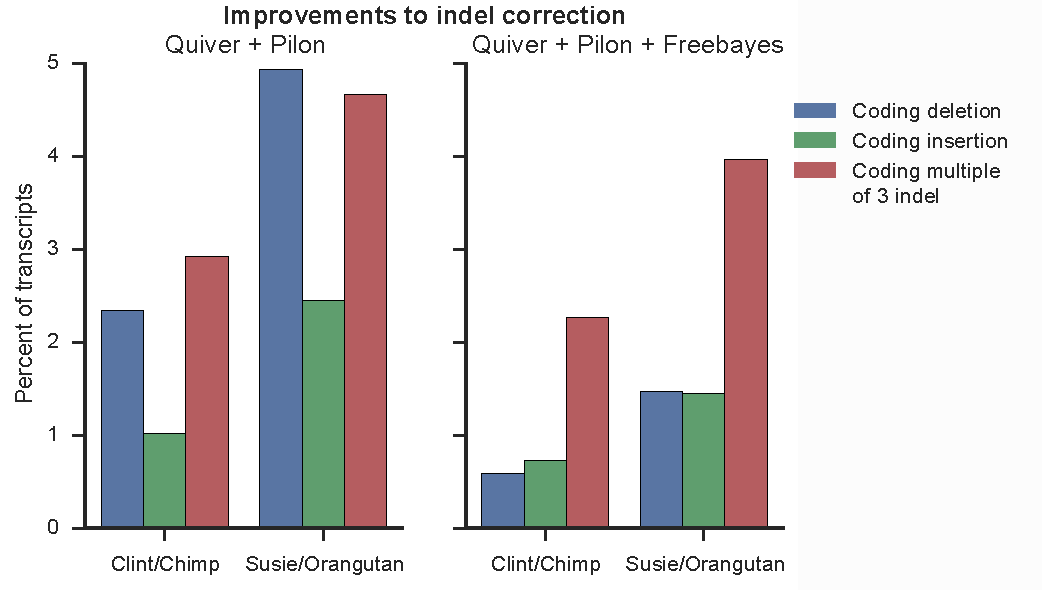
\includegraphics[width=\textwidth,height=\textheight,keepaspectratio]{primate_indels.pdf}
\caption{Primate Coding Indels}
The rate of transcripts with coding indels seen in the consensus gene sets for the SMRT primate assemblies are shown with Quiver and Pilon correction (left), and subsequent Freebayes  \citep{garrison2012haplotype}-based correction (right). Freebayes correction was not performed on GSMRT5 (gorilla). Coding indels are measured by pairwise translated BLAT alignments of a transcript to its ortholog in human. SMRT assemblies show a systematic overrepresentation of coding deletions. After Freebayes correction, the rate of insertions to deletions is roughly equal and lower than the rate of multiple of 3 indels, which is the expected result due to purifying selection.
\label{supp_fig:primate_indels}
\end{figure}

\begin{figure}
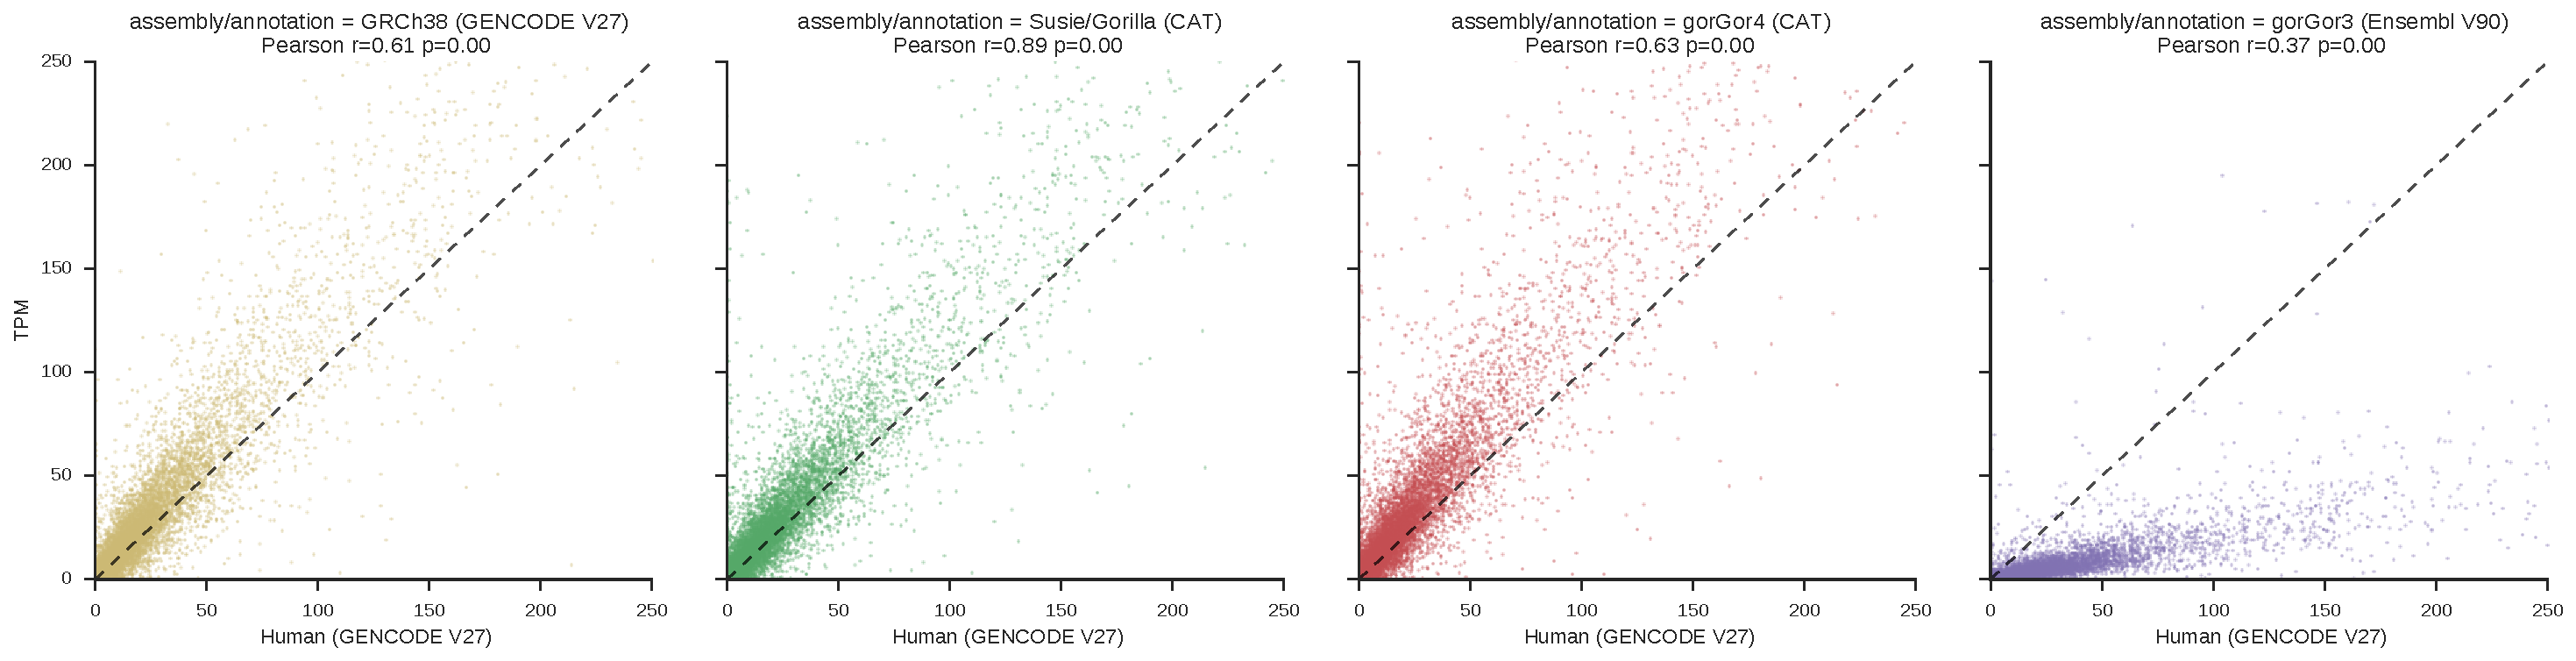
\includegraphics[width=0.8\paperwidth,keepaspectratio]{gorilla_kallisto.pdf}

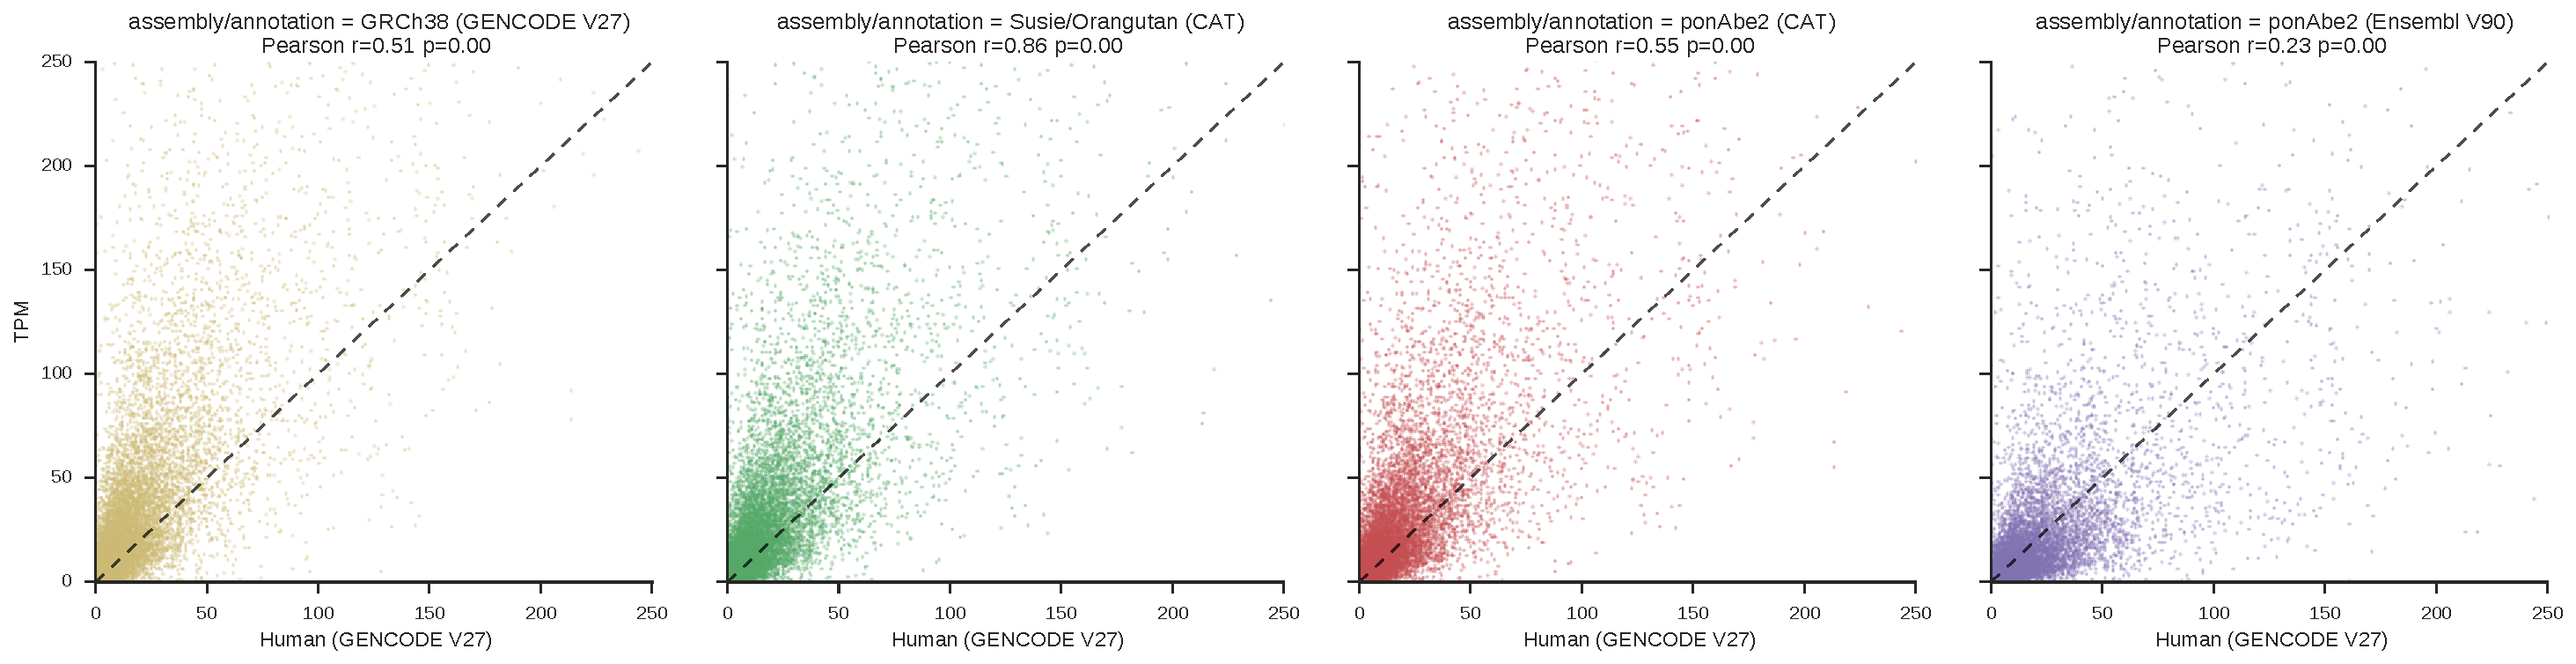
\includegraphics[width=0.8\paperwidth,keepaspectratio]{orangutan_kallisto.pdf}
\caption{Cross-species RNA-seq expression estimates}

Gorilla and orangutan iPSC RNA-seq are compared to human iPSC RNA-seq using a variety of annotation and assembly combinations. All comparisons were performed with Kallisto. Cross-species comparison was used by tracking gene common names, and only protein-coding genes were considered. Because the pre-release of Ensembl V91 provided to us lacked common names, we used V90. Ensembl V90 annotation is on gorGor3, so that genome was used. The x-axes in all plots are the TPM of human iPSC data mapped to GENCODE V27. The y-axes in all plots are the TPM of species-specific iPSC RNA-seq mapped to the assembly/annotation pair in the title. In all cases, using the newest version of the assemblies with CAT provides the highest correlation.
\label{supp_fig:primate_expression}
\end{figure}

\begin{figure}

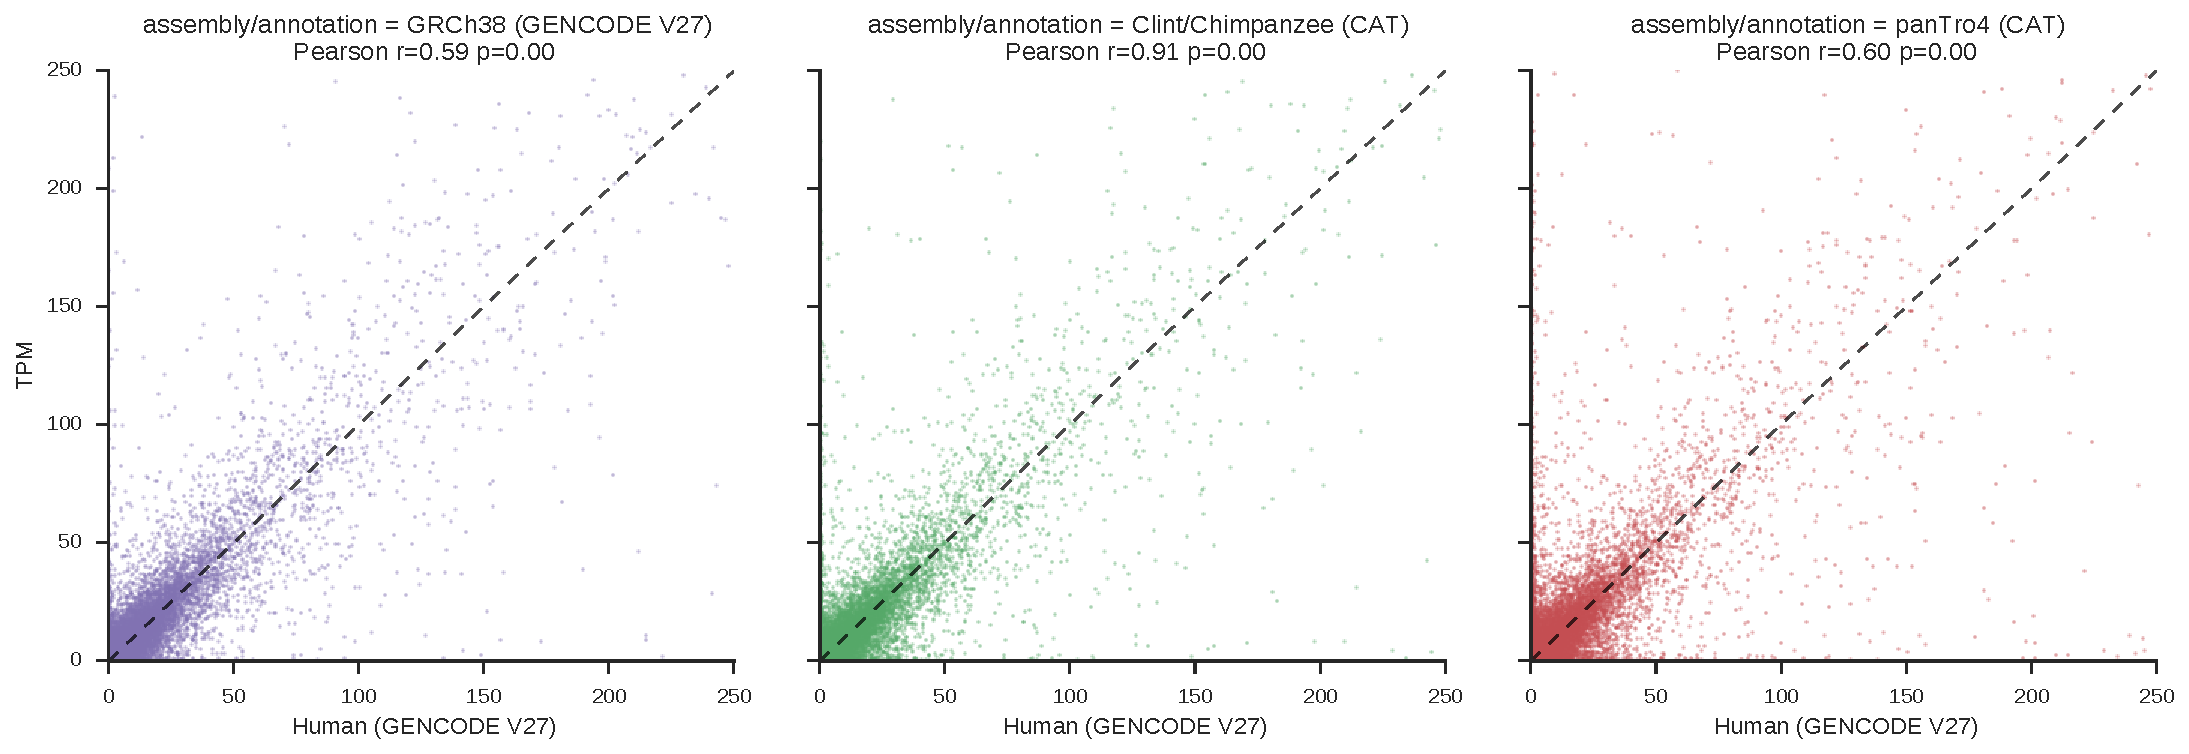
\includegraphics[width=0.8\paperwidth,keepaspectratio]{chimp_kallisto_transcripts.pdf}

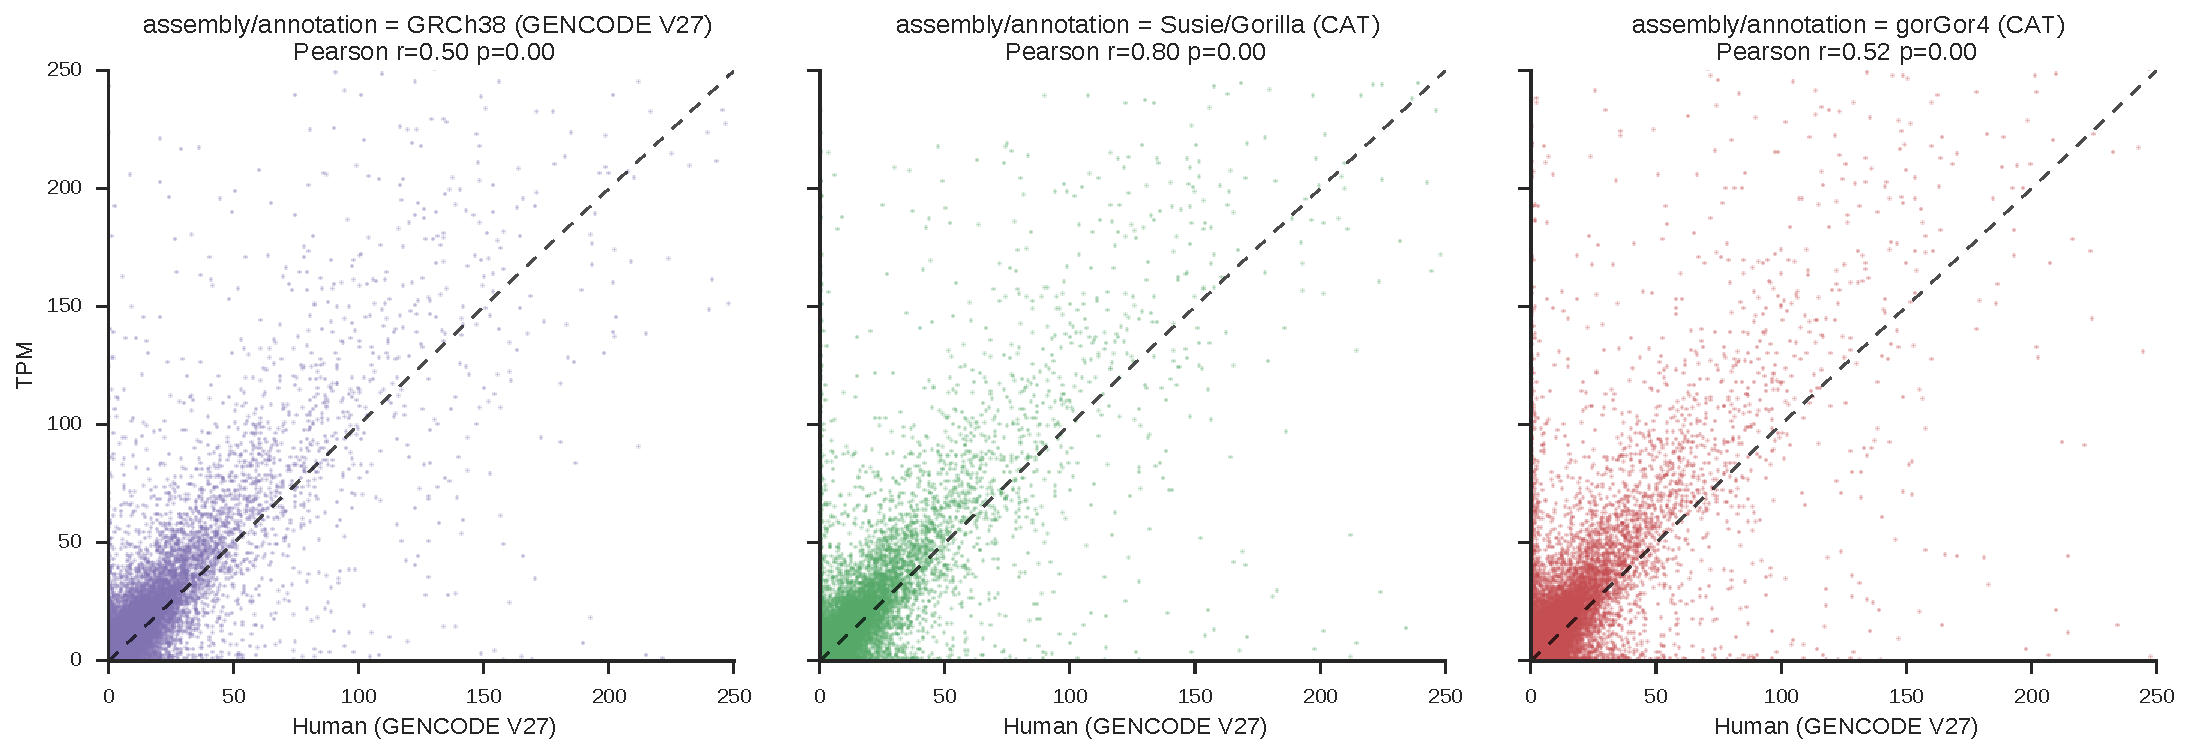
\includegraphics[width=0.8\paperwidth,keepaspectratio]{gorilla_kallisto_transcripts.pdf}

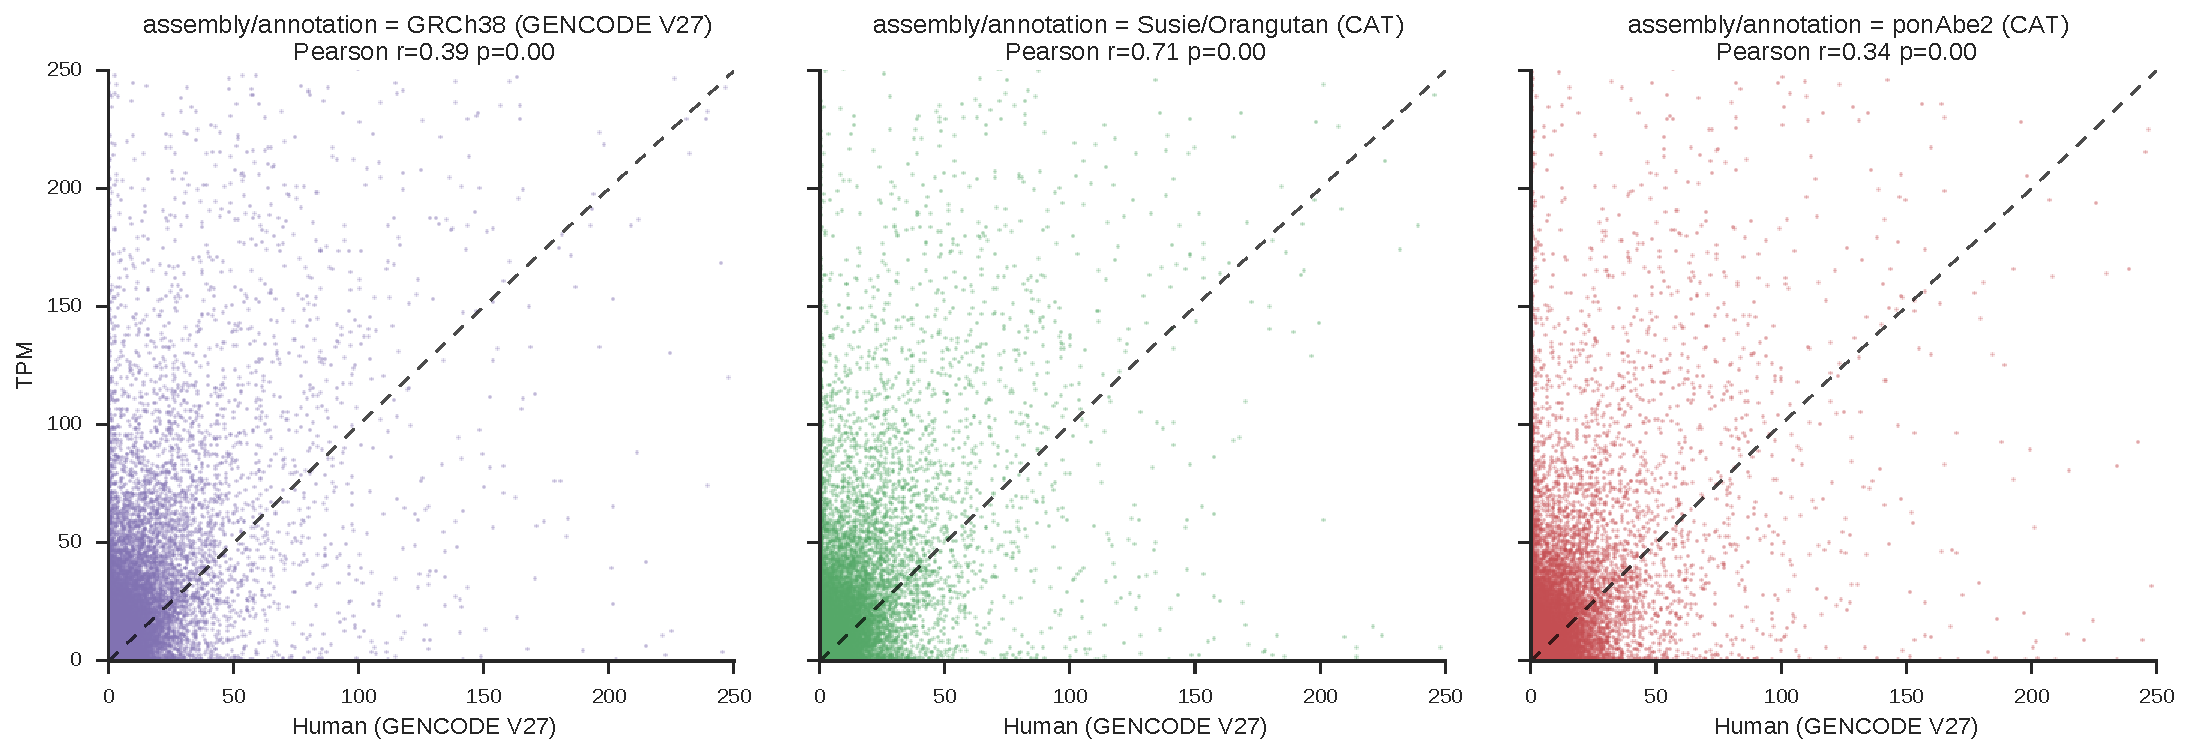
\includegraphics[width=0.8\paperwidth,keepaspectratio]{orangutan_kallisto_transcripts.pdf}

\caption{Cross-species RNA-seq isoform expression estimates}
The same analysis as in Figure \ref{fig:primate}D and Supplemental Figure \ref{supp_fig:primate_expression} was performed on the isoform level. For this analysis Ensembl was not included because we lacked a mapping of isoform IDs between the Ensembl annotation set and GENCODE. Only protein-coding isoforms were considered. The highest correlation is seem in CAT annotation of SMRT genomes, although correlation falls off considerably as phylogenetic distance increases from chimpanzee to orangutan.

\label{supp_fig:primate_transcript_expression}
\end{figure}

\begin{figure}
\centering
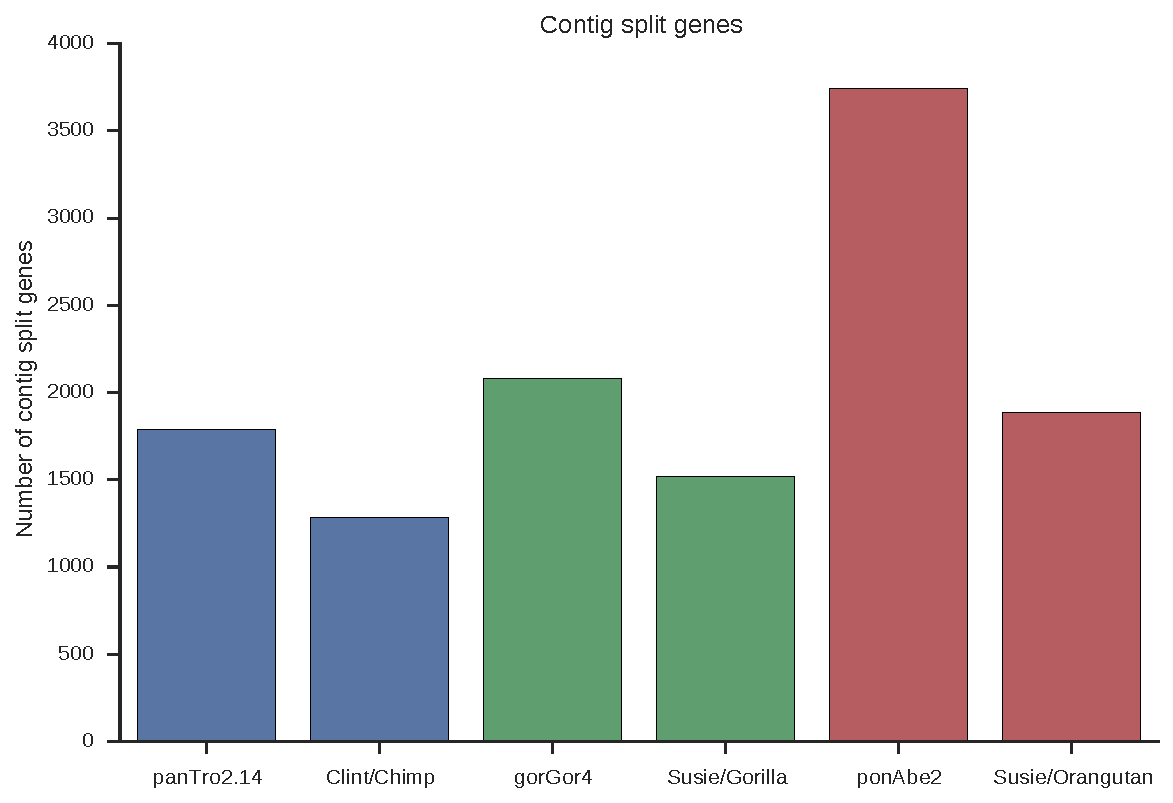
\includegraphics[width=\textwidth,height=\textheight,keepaspectratio]{split_genes.pdf}
\caption{Primate Split Genes}
\label{supp_fig:primate_split_genes}
Split gene analysis looks for transcript projections after paralog resolution that map to multiple contigs. This provides a metric for assembly contiguity. Despite the PacBio assemblies not being in chromosome-sized pieces, fewer split genes are detected, suggesting that most contig breaks are not in genic regions.
\end{figure}

\begin{figure}
\centering
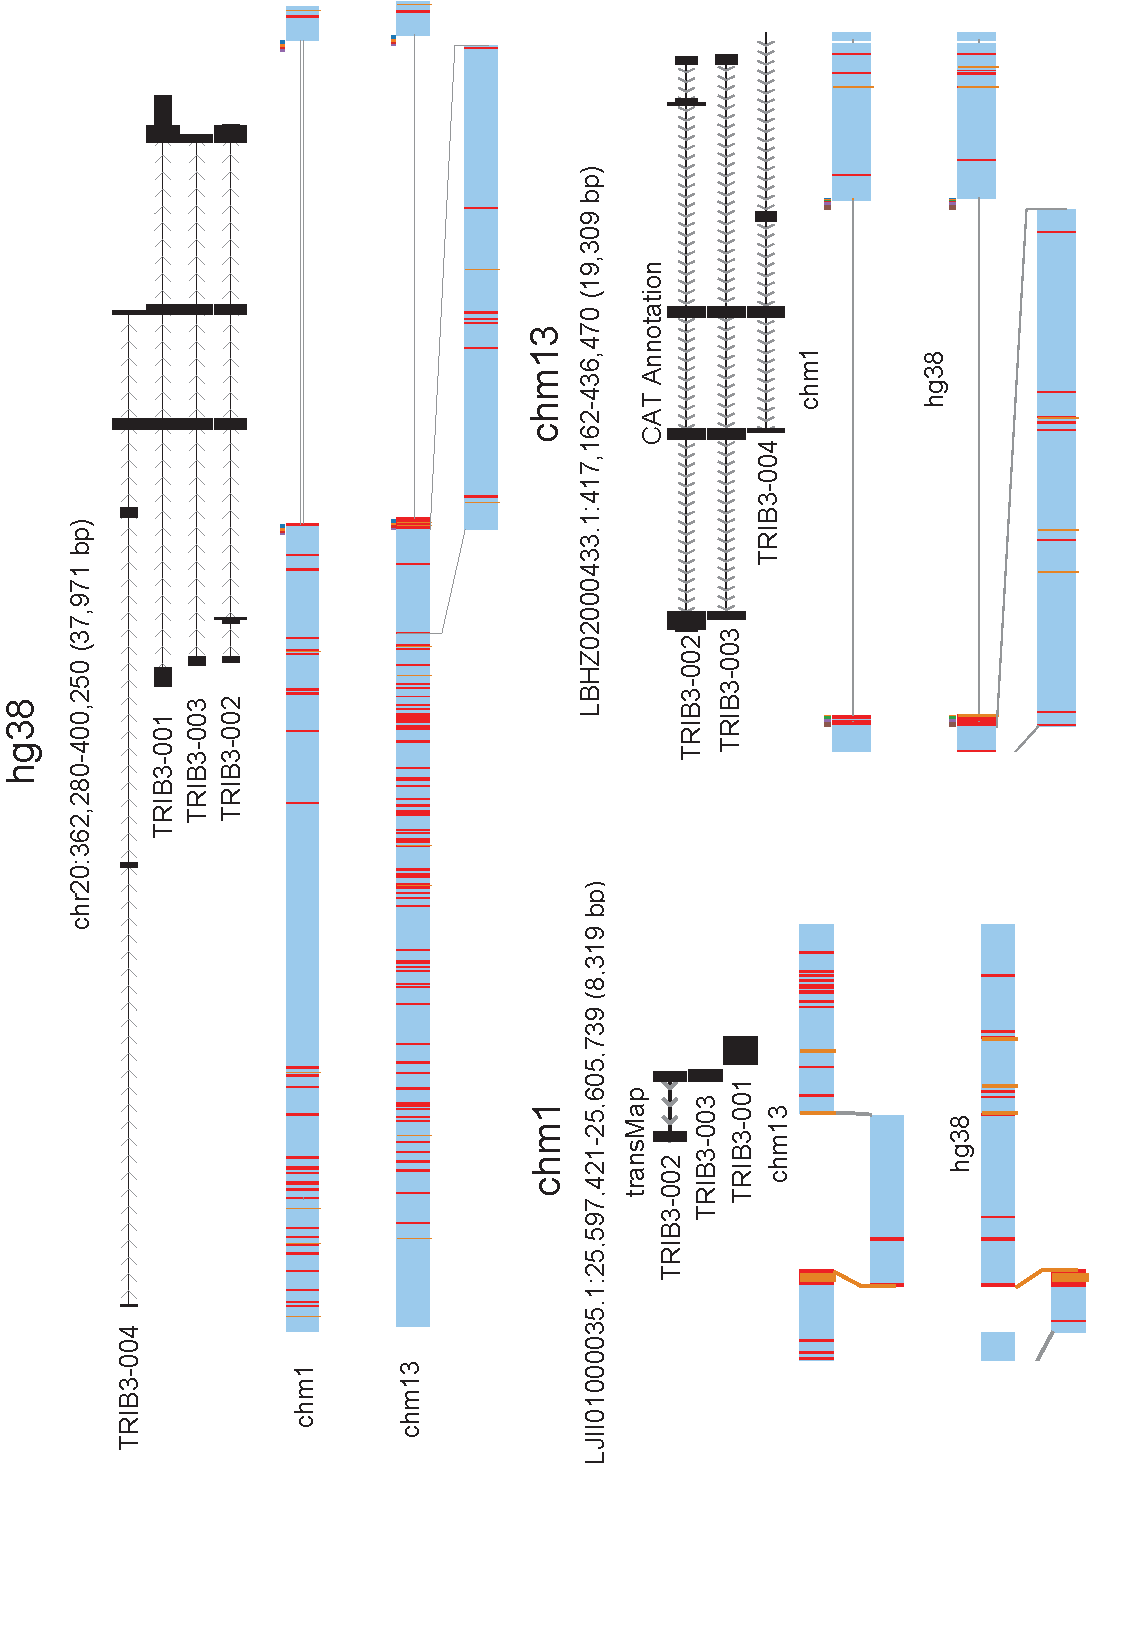
\includegraphics[width=0.8\textwidth,height=0.7\textheight,keepaspectratio]{trib3_full.pdf}
\caption{\textit{TRIB3} example}
The CHM1 structural variant in figure 4 is shown here from all perspectives. In CHM1, the short transMaps for the few remaining exons are filtered out and do not end up in the annotation set. In contrast, CAT annotated 3/4 of the isoforms. This figure shows the power of the UCSC assembly hub for evaluating structural variants by being able to view the alignment from any species present.
\label{supp_fig:trib3}
\end{figure}

\begin{figure}
\centering
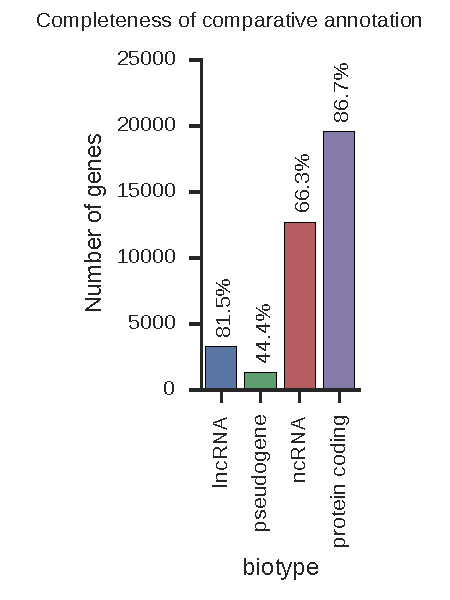
\includegraphics[]{rat_completeness.pdf}
\caption{Rat completeness}
The number of genes comparatively identified in the rn6 assembly from mm10 GENCODE VM11, broken down by simplified biotypes. The percentages on top are the percent of the total genes in each simplified biotype present in VM11. While a large portion of protein-coding genes are identified, much fewer lncRNAs and other noncoding biotypes are identified.
\label{supp_fig:rat_completeness}
\end{figure}

\begin{figure}
\centering
\makebox[\textwidth]{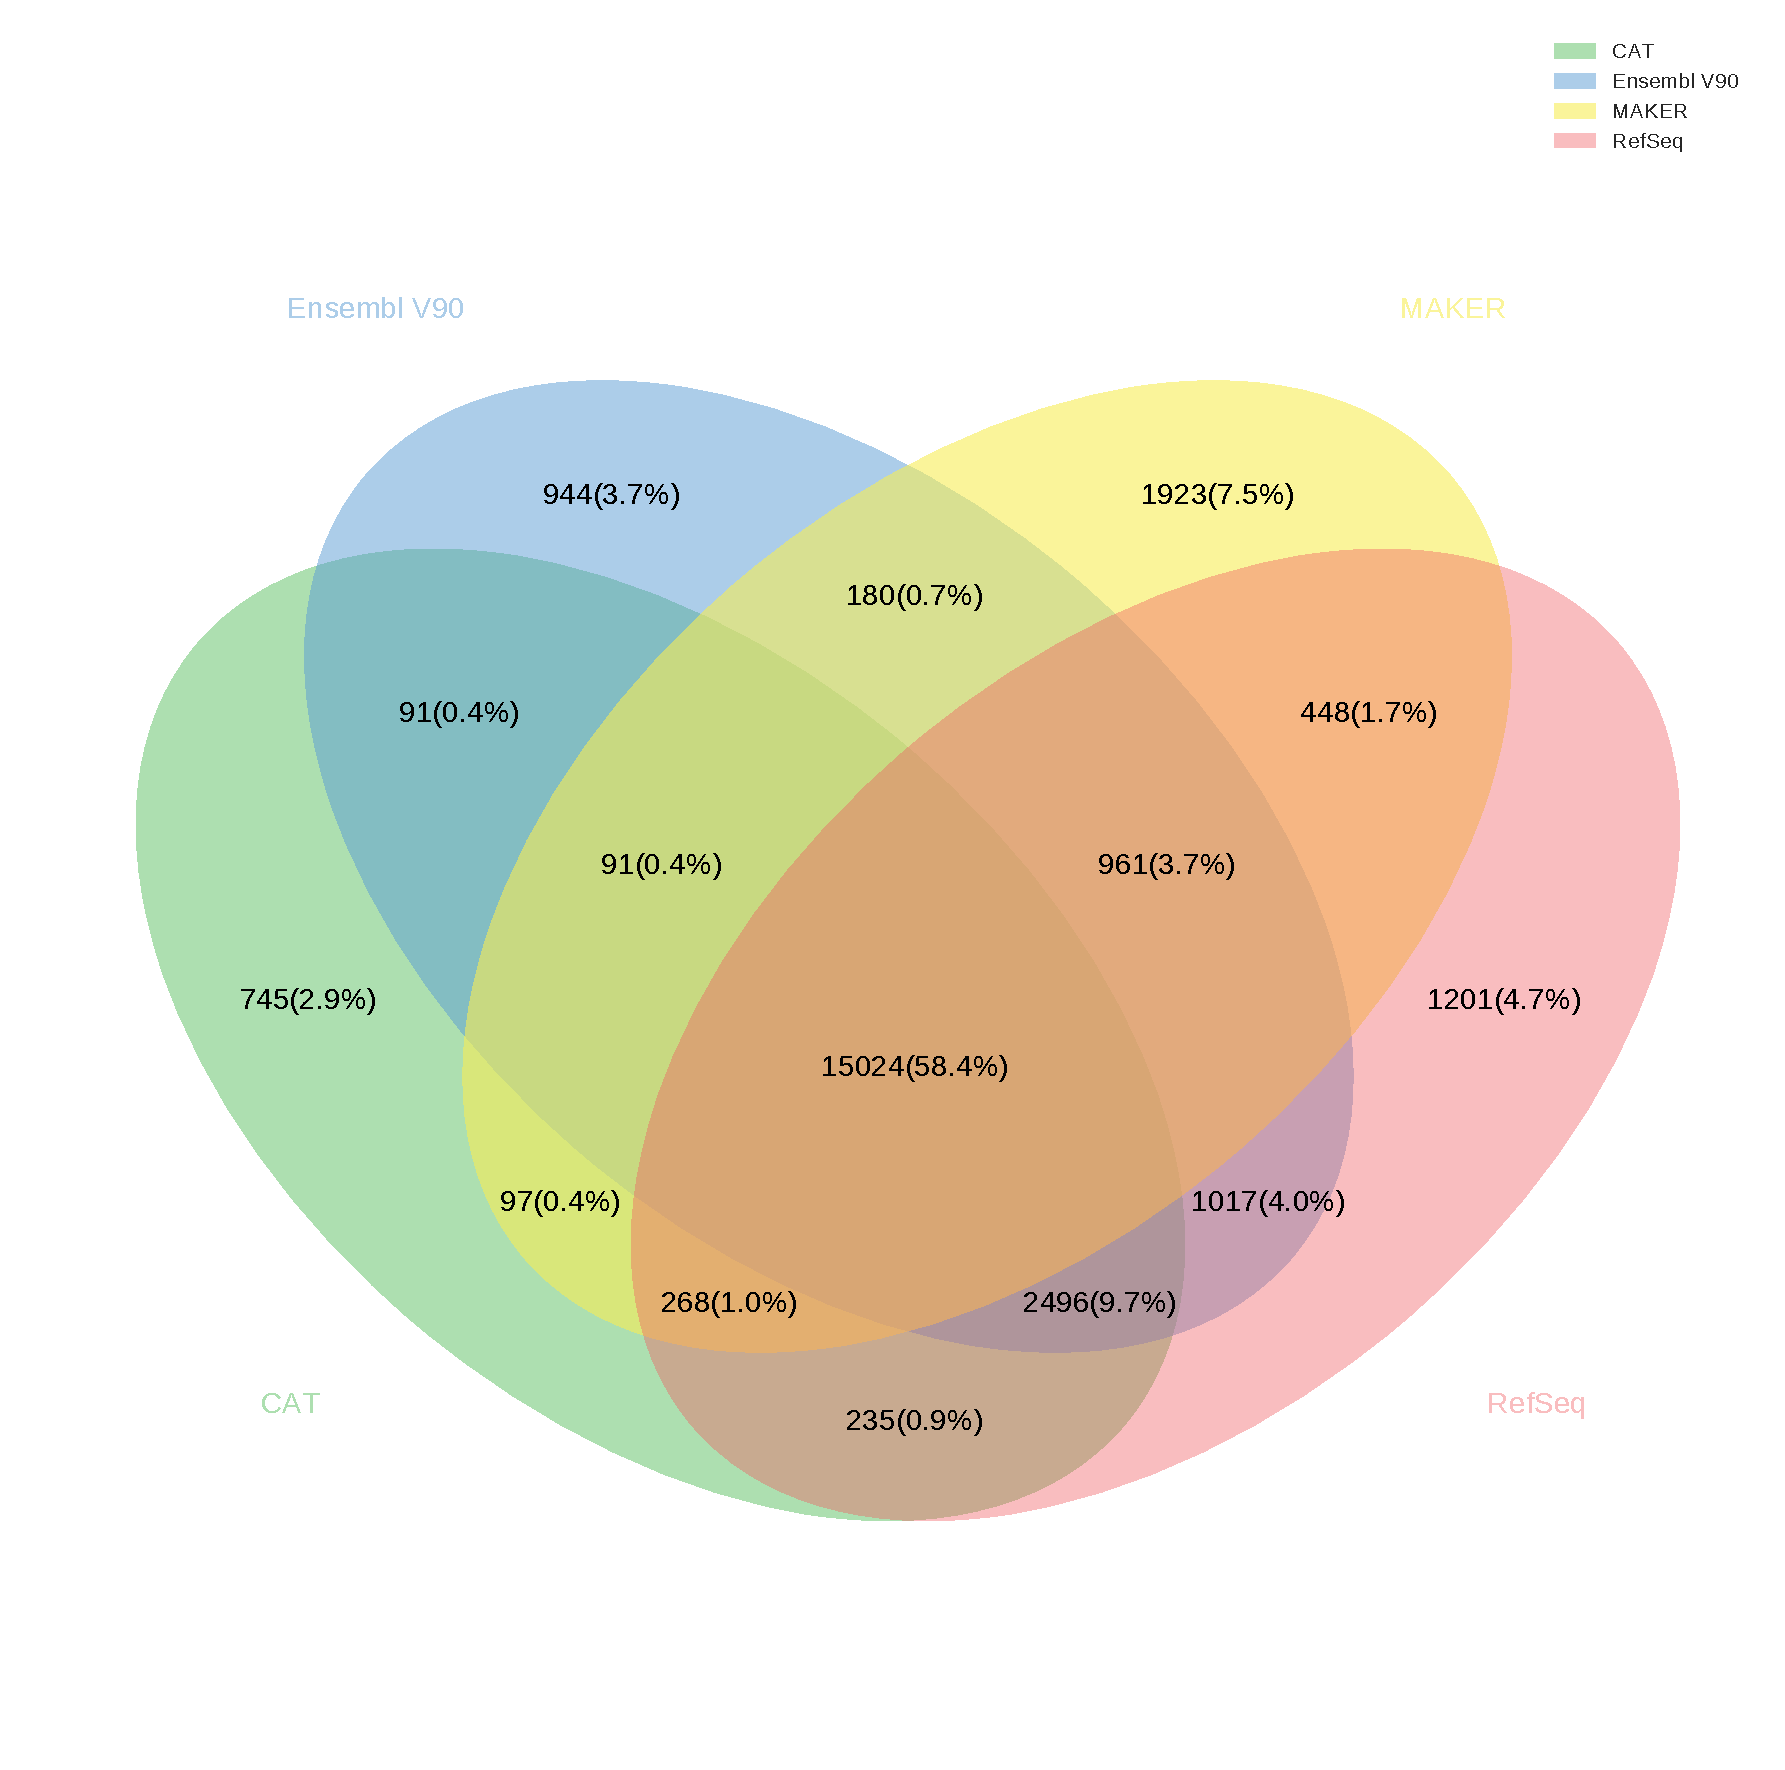
\includegraphics[width=0.8\paperwidth]{transcript_clusters.pdf}}
\caption{Rat Locus Venn Diagram}
Gene loci were compared between CAT, Ensembl V90, MAKER and RefSeq on rat rn6. Loci were clustered using the Kent tool clusterGenes, which requires exonic overlap on the same strand. Only 15,179 loci are shared between all sets.
\label{supp_fig:rat_locus_venn}
\end{figure}

\begin{figure}
\centering
A)
\makebox[\textwidth]{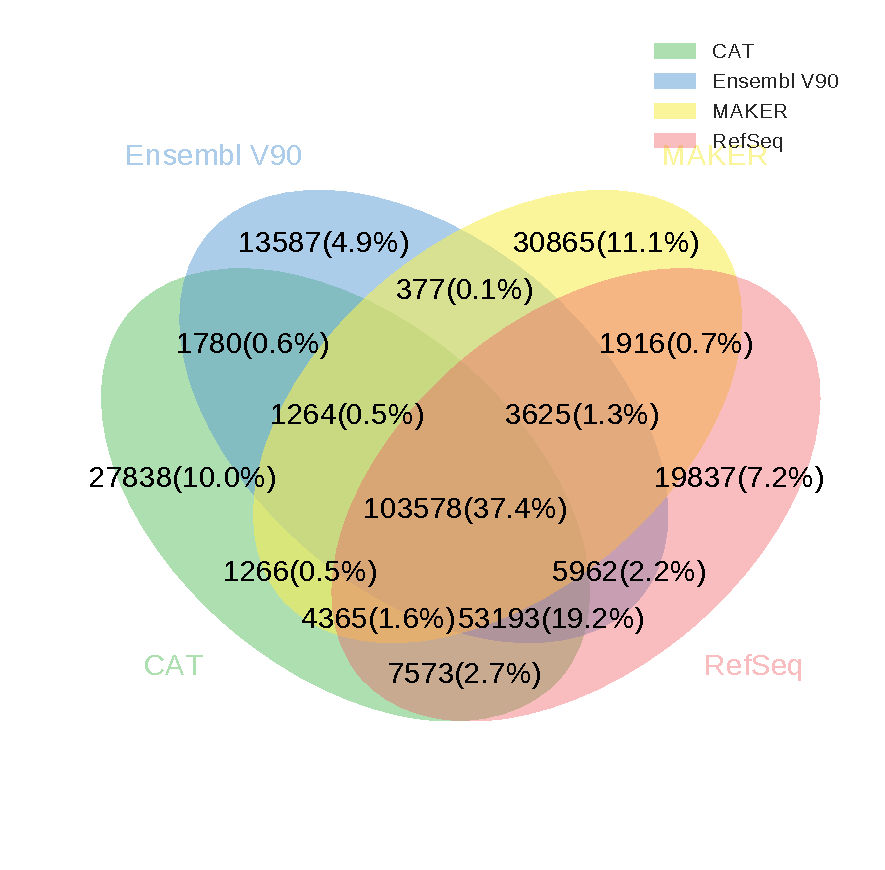
\includegraphics[width=0.45\paperwidth]{cds_intron_venn.pdf}}
B)
\makebox[\textwidth]{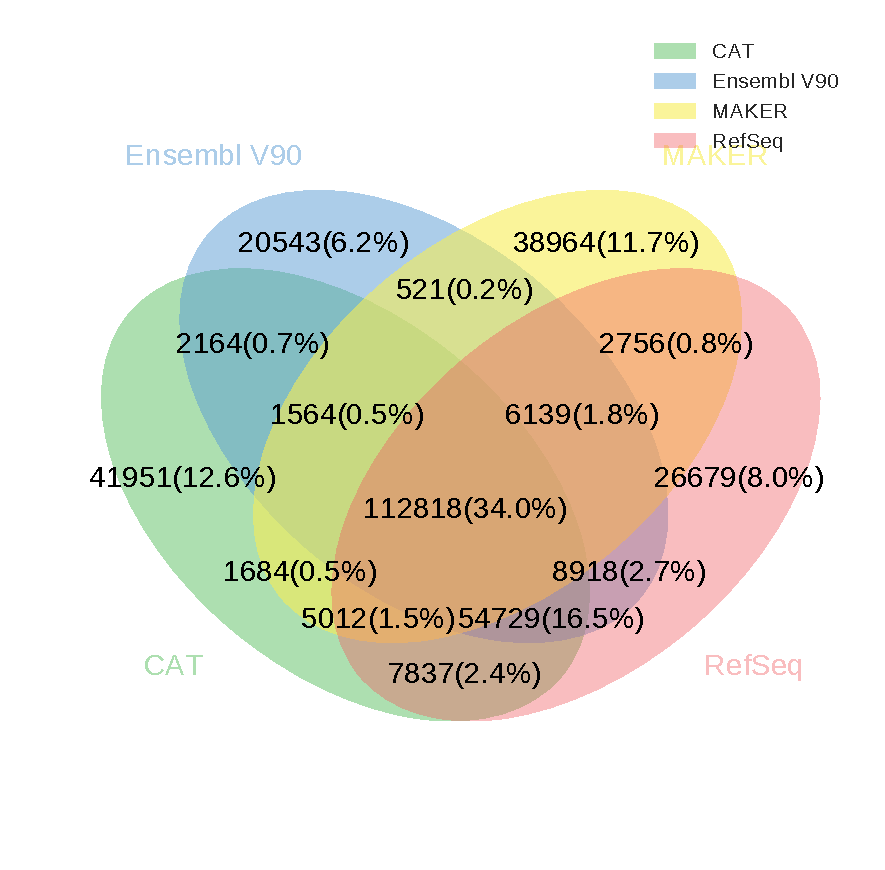
\includegraphics[width=0.45\paperwidth]{cds_exon_venn.pdf}}
\caption{Rat Exon/Intron Support Venn Diagram}
CDS Intron (left) and CDS exon (right) interval exact matches were compared between CAT, Ensembl V90, MAKER and RefSeq on rat rn6. MAKER had the highest proportion of unsupported exons and introns, followed by CAT. Only 37.0\% and 34.0\% of introns and exons respectively are present in all four annotation sets.
\label{supp_fig:rat_exon_intron}
\end{figure}

\begin{figure}
\centering
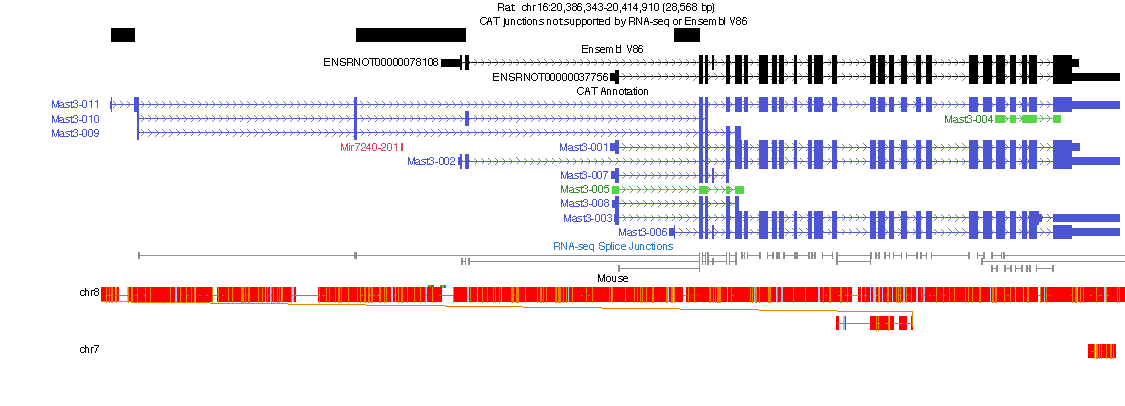
\includegraphics[width=\textwidth,height=\textheight,keepaspectratio,angle=90]{mast3_example.pdf}
\caption{Unsupported junctions example}
The rat gene Mast3 has two annotated isoforms in Ensembl supported by RNA-seq. CAT annotation added 9 new isoforms, two of which had unsupported junctions. These new annotations reveal an upstream transcription initiation site supported by RNA-seq. 
\label{supp_fig:unsupported_junctions}
\end{figure}

\begin{table}
\centering
\begin{tabular}{|l|l|}
 \hline
Genome & Number of BUSCO genes missing \\ \hline
\textit{Mus pahari}      & 38 \\ \hline
Rat (rn6)      & 99 \\ \hline
Rhesus (rheMac3)   & 138 \\ \hline
Chimpanzee (panTro4) & 90 \\ \hline
Human (hg19)     & 26 \\ \hline
Gorilla (gorGor3)  & 184 \\ \hline
Orangutan (ponAbe2) & 133 \\ \hline
Cat (felCat8)    & 95 \\ \hline
Elephant (loxAfr3)  & 114 \\ \hline
Rabbit (oryCun2)   & 147 \\ \hline
Dog (canFam3)    & 90 \\ \hline
Sheep (oviAri3)   & 162 \\ \hline
Cow (bosTau8)    & 93 \\ \hline
\end{tabular}
\caption{BUSCO genes missing in 13 mammal annotation}
BUSCO  \citep{simao2015busco} was used to quantify the number of core key genes missing in the CAT annotation of 13 mammalian genomes. For this analysis, the mammalian odb\_9 set of 4,104 genes was used. BUSCO genes represent core housekeeping genes present at single copy across long evolutionary distance. On average, 108 BUSCO genes (2.63\%) are missing in each genome. Only three BUSCO genes (EOG090A0GHJ, EOG090A05ND, and EOG090A04MN) were missing in all 13 genomes.
\label{supp_table:busco}
\end{table}

\begin{center}
\small
\captionof{table}{SRA RNA-seq accessions}
\label{supp_table:rnaseq_sra_table}
\begin{longtable}{|p{0.15\textwidth}|p{0.65\textwidth}|p{0.2\textwidth}|} \hline
Species  & SRA Accessions & Tissues \\ \hline
Rat    & SRR1041777, SRR1768421, SRR1768443, SRR1768444, SRR299123, SRR636875, SRR636876, SRR636877, SRR636925, SRR636926, SRR636927, SRR636970, SRR636971, SRR636972                                                                                                                                          & Mixed, testis, liver, kidney, brain                                          \\ \hline
Orangutan & SRR306792, SRR2176206, SRR2176207                                                                                                                                                                                                       & Brain, testis                                                     \\ \hline
Gorilla  & SRR832925, SRR3053573, SRR306809, SRR306803, SRR306804, SRR306801, SRR306807, SRR306810, SRR306805, SRR306806, SRR306802, SRR306800, SRR306808                                                                                                                                                 & Brain, 20 tissue pool                                                 \\ \hline
Chimp   & SRR2040584, SRR2040585, SRR2040586, SRR2040587, SRR2040588, SRR2040589, SRR2040590, SRR2040591, SRR3711187, SRR3711188, SRR873622, SRR873623, SRR873624, SRR873625                                                                                                                                       & brain, heart, liver, testis, 8 week old iPSC derived neurons, undifferentiated iPSC                  \\ \hline
Rhesus  & SRR306784, SRR306786, SRR306785, SRR2040593, SRR306783, SRR306787, SRR306780, SRR306778, SRR306790, SRR2040595, SRR2040594, SRR2040592, SRR306788, SRR306782, SRR306789, SRR306777, SRR306779, SRR306781                                                                                                                    &  Kidney, liver, heart, brain, testis                                                          \\ \hline
Human   & ERR579132, ERR579133, ERR579134, ERR579135, ERR579136, ERR579137, ERR579138, ERR579139, ERR579140, ERR579141, ERR579142, ERR579143, ERR579144, ERR579145, ERR579146, ERR579147, ERR579148, ERR579149, ERR579150, ERR579151, ERR579152, ERR579153, ERR579154, ERR579155                                                                                     & Ovary, tonsil, fallopian tube, placenta, endometrium, rectum, skeletal muscle, liver, fat, colon, smooth muscle, lung \\ \hline
Sheep   & SRR1653601, SRR1561187, SRR1561150, SRR1265856, SRR1536790, SRR1561171, SRR1265854, SRR1561367, SRR1561365, SRR1653570, SRR1653598, SRR1653597, SRR1266019, SRR1265849, SRR1653600, SRR1656805, SRR1561366, SRR1653594, SRR1561196, SRR1265855, SRR1653596, SRR1536788, SRR1266022, SRR1561156, SRR1266018, SRR1561195, SRR1536770, SRR1266020                                                 &   Liver, brain, blood                                                          \\ \hline
Cow    & SRR2960011, SRR2960020, SRR2960008, SRR2960010, SRR2960012, SRR2960016, SRR2960006, SRR2960015, SRR2960025, SRR2960003, SRR2960022, SRR2960029, SRR2960030, SRR2960017, SRR2960032, SRR2960005, SRR2960027, SRR2960007, SRR2960036, SRR2960026, SRR2960035, SRR2960004, SRR2960002, SRR2960034, SRR2960013, SRR2960001, SRR2960021, SRR2960019, SRR2960009, SRR2960024, SRR2960014, SRR2960031, SRR2960033, SRR2960023, SRR2960028, SRR2960018 &  Liver, udder                                                          \\ \hline
Elephant & SRR1041765, SRR975189, SRR975188, SRR3222430                                                                                                                                                                                                  &    Fibroblast                                                        \\ \hline
Rabbit  & SRR636919, SRR636872, SRR636964, SRR636871, SRR636920, SRR636965                                                                                                                                                                                        &     Liver, kidney, brain                                                       \\ \hline
Cat    & SRR3200450, SRR3200448, SRR3200449, SRR3200453                                                                                                                                                                                                 &   Fetus, lung, liver                            \\ \hline              
\end{longtable}
Publicly available RNA-seq obtained via SRA for annotations performed in this paper. 
\end{center}

\end{document}

